\documentclass[egregdoesnotlikesansseriftitles]{scrartcl}

\usepackage[T1]{fontenc}
\usepackage[utf8]{inputenc}

\usepackage{amsmath}
\usepackage{amssymb}
\usepackage[greek,english]{babel}
\usepackage{caption}
\usepackage{dcolumn}
   \newcolumntype{d}[1]{D{.}{.}{#1}}
\usepackage{float}
\usepackage{graphicx}
\usepackage[hidelinks,pdfusetitle]{hyperref}
   \urlstyle{rm}
\usepackage[authoryear]{natbib}
\usepackage{pdflscape}
\usepackage{soul}
\usepackage{subcaption}
\usepackage{xcolor}

\deffootnote{1.5em}{1em}{\makebox[1.5em][l]{\thefootnotemark}}
   \setlength{\skip\footins}{1.5em}
   \setlength{\footnotesep}{1em}

\begin{document}
\thispagestyle{empty}
\renewcommand{\thefootnote}{\fnsymbol{footnote}}
\begin{center}
   {\LARGE Winter is Coming}\\\vspace{2ex}
   {\Large How Laypeople Think About Different Kinds of Needs}\\\vspace{4ex}
   {\large Alexander Max Bauer,$^{a}$\footnotemark[1] Jan Romann,$^{b}$\\ Mark Siebel,$^a$ and Stefan Traub$^c$}\\\vspace{2ex}
   \textsl{\footnotesize $^{a}$Department of Philosophy, University of Oldenburg, Oldenburg, Germany}\\\vspace{0.5ex}
   \textsl{\footnotesize $^{b}$Faculty of Technology, University of Applied Sciences Emden/Leer, Emden, Germany}\\\vspace{0.5ex}
   \textsl{\footnotesize $^{c}$Department of Economics, Helmut-Schmidt-University, Hamburg, Germany}\\\vspace{2ex}
\end{center}

\vspace{\fill}\noindent\textbf{Abstract:} Needs play a key role in many fields of social sciences and humanities, ranging from normative theories of distributive justice to conceptions of the welfare state.
Over time, different conceptions of what counts as a need (i.\,e., what is considered a normatively relevant need) have been proposed.
Many of them include (in one way or the other) needs for survival, decency, belonging, and autonomy.
Little work has been done on how these kinds of needs are evaluated in terms of their significance for distributive justice.
To begin closing this gap, we investigate the role of the four aforementioned kinds of needs for impartial observers.
We do so in two empirical studies.
The first study asks participants to evaluate the importance of each of the four kinds of needs separately.
We find that different levels of importance are attributed to the kinds of needs, which places them in a hierarchy.
The second study asks participants to make distributive decisions.
Results further support the hierarchy found in the first study and, additionally, reveal that participants tend to make coherent allocation decisions.\\[0.5ex]

\noindent\textbf{Keywords:} Basic Needs, Coherence, Distributive Justice, Equality, Equity, Rationality

\footnotetext[1]{Corresponding author.
Department of Philosophy, University of Oldenburg, Ammerl{\"a}nder Heerstra{\ss}e 114--118, 26129 Oldenburg, Germany, \href{mailto:alexander.max.bauer@uni-oldenburg.de}{alexander.max.bauer@uni-oldenburg.de}.
Telephone: +49 (0)441 798 2034.
The authors were members of the research group ``Need-Based Justice and Distributive Procedures'' (FOR 2104) funded by the German Research Foundation (DFG Grants SI $1731/2-2$, TR $458/6-2$).
We are indebted to the support and input throughout all project phases by participants of FOR 2104 meetings.}

\renewcommand{\thefootnote}{\arabic{footnote}}\setcounter{footnote}{0}
\newpage


%%%%%%%%%%%%%%%%
% INTRODUCTION %
%%%%%%%%%%%%%%%%
\section{Introduction}\label{sec:introduction}
Imagine that you were living in a cottage that you heated exclusively with firewood.
Spring has given way to summer, summer has given way to autumn – and temperatures are starting to fall.
Winter is coming, and, unfortunately, you are short on firewood.
And now imagine that without additional firewood it would get so cold in your hut that you would probably become life-threateningly ill.

In this case, your physical integrity---something that pretty much all authors can agree counts as a basic need---is seriously threatened.
Such needs have played a role in philosophy since antiquity (see, e.\,g., \citealt{poelzler_basic_2021}, who interprets Aristotle's reflections on \textgreek{ἀναγκαῖον} in his \textit{Metaphysics} as related to basic needs; \citealt[1015a20--1015b15]{aristotle_metaphysics_1933}), they feature in the \textit{Acts of Luke}, when the Christian community is described (see \citealt[p. 302f.]{bauer_gerechtigkeit_2019}; \citealt[p. 141f.]{luke_apostelgeschichte_2016}), and they have repeatedly been emphasized in the history of thought (e.\,g., \citealt{marx_kritik_1969}). In the last century, then, psychology (e.\,g., \citealt{maslow_theory_1943}, \citealt{alderfer_existence_1972}) and philosophy (e.\,g., \citealt{thomson_need_1987}, \citealt{miller_principles_1999}, \citealt{hamilton_political_2003}; for overviews see \citealt{brock_needs_2019}, \citealt{miller_needs_2020}, \citealt{siebel_need-based_2020}, as well as \citealt{poelzler_basic_2021}), among some other fields,\footnote{For perspectives from philosophy, psychology, sociology, political science, and economics, see \cite{kittel_need-based_2020}.} found new interest in the topic, and needs have gained new weight as a cornerstone of the welfare state (see, e.\,g., \citealt{esping-andersen_three_1990}).

Authors have developed countless theories of what counts as a basic need.
Few things obtain such an unanimous approval as---the above sketched---physical integrity.
In the course of this paper, we identify a \textit{hierarchy} of four kinds of needs that are recurring in the literature: survival, decency, belonging, and autonomy.
We ask whether these needs are perceived as having different degrees of importance (first indications that this might indeed be the case are provided by the studies of \citealt{poelzler_typicality_2022} as well as \citealt{bauer_needs_forthcoming}).
To test this, we designed and conducted two empirical studies.

The first study elicits absolute need evaluations.
Here, participants were first given short vignettes presenting our four types of needs in a hypothetical context.
Each vignette was introduced with an illustration of the hypothetical situation.
Then, for each of them, participants had to indicate how important they consider the need in question to be.
We find that different levels of importance are attributed to the kinds of needs, effectively placing them in a clear hierarchy.

The second study sheds light on relative need evaluations.
Here, too, participants were first familiarized with vignettes of the four kinds of needs and the corresponding illustrations.
Then they were presented with cases showing two people.
Cases varied as to what kind of need the two people experience.
The participants' task was to distribute a scarce good between these two hypothetical people as impartial decision-makers.
As an additional within-participants variation, we altered whether both persons contributed equally or unequally to the amount available for distribution.
This way, we investigate whether productivity has an effect on the decisions.
Our findings further support the hierarchy we found in the first study.
Moreover, productivity has an effect on participants' decisions.
In addition, we are able to observe that our participants' need evaluations are coherent in terms of being additive.

The rest of this paper is structured as follows.
Section \ref{sec:literature} gives a review of the relevant literature.
Section \ref{sec:study_1} reports our first and Section \ref{sec:study_2} our second study.
Section \ref{sec:conclusion} concludes the paper.


%%%%%%%%%%%%%%
% LITERATURE %
%%%%%%%%%%%%%%
\section{Literature Review}\label{sec:literature}
As has been pointed out recently, e.\,g., by \cite{kittel_impact_2020} and \cite{bauer_need_2022}, needs are not only relevant for normative reflections, but have also been the subject of numerous empirical studies.
Think, for example, of early empirical social choice (e.\,g., \citealt{yaari_dividing_1984}) and what followed from it (for a review, see \citealt{gaertner_empirical_2012}).
At least since the beginnings of motivational psychology (e.\,g., \citealt{williams_multi-dimensional_1989}) they are also to be found in the field of psychology (for a review, see \citealt{diederich_identifying_2020}).
Population surveys have also revealed that basic needs play a role in people's ideas of justice (e.\,g., \citealt{reeskens_equity_2013}, \citealt{hulle_measuring_2018}).
Incentivized economic experiments have shown that needs influence subjects' decisions (e.\,g., \citealt{branas_poverty_2006}, \citealt{cappelen_needs_2013}).
There were also attempts to bring real needs into the laboratory (e.\,g., \citealt{kause_selfish_2018}).
Hence, our studies and their implications regarding the concept of need potentially touch on many different fields of research.

The concept of need has been defined in different ways.
Generally, needs may be attributed by the locution ``\textit{S} needs \textit{x} in order to $\Phi$''.
In the context of justice, the expression at \textit{S} typically refers to persons, but we may equally think of households, companies, and so fourth.
The term at \textit{x} designates the object of a need, viz., the thing needed.
This can be a material resource, but also other goods, such as personal relationships.
The expression at $\Phi$ stands for the goal to be achieved with the object of the need, which may be an action, a status, an opportunity, and so forth.
In any case, by claiming that \textit{S} needs \textit{x} in order to $\Phi$, it is stated that \textit{x} is \textit{necessary} for \textit{S} to achieve $\Phi$.

A need claim can be \textit{purely instrumental}, such as ``She needs a hammer in order to knock in the nail''.
Such a claim is morally neutral in itself; its moral relevance depends, among other things, on the moral relevance of the goal involved.
Many authors tell such instrumental needs from \textit{categorical} (absolute or intrinsic) ones.
Categorical needs are distinguished from mere wants, wishes, or desires---either through some objective criterion (\citealt{brock_needs_2005}, \citealt{thomson_fundamental_2005}, \citealt{weale_needs_1998}, \citealt{wringe_needs_2005}) or through some inter-subjective process (\citealt{kelsen_was_2016}, \citealt{hamilton_political_2003}, \citealt{miller_principles_1999}). 
Furthermore, they are assumed to bear a normative force since what they aim at is regarded as something that ought to be realized.
In other words, they are taken to be ``necessary, indispensable, or inescapable, at least with respect to some important goals'' (\citealt[par. 37]{brock_needs_2019}).
The overarching goal most commonly used to characterize categorical needs is avoidance of harm, or in positive terms, living a decent life (see, i.\,a., \citealt{frankfurt_necessity_1984}, \citealt{miller_social_1976,miller_principles_1999}, \citealt{thomson_need_1987,thomson_fundamental_2005}, \citealt{wiggins_needs_1987,wiggins_what_1998}).

There are quite a few distinctions between categorical needs to be found in the literature.\footnote{Note that, in the course of history, a variety of lists of such needs have been suggested, specifying what does count as a basic need (e.\,g., \citealt{doyal_theory_1991}, \citealt{braybrooke_meeting_1987}, \citealt{nussbaum_aristotelian_1990}).
Others have opposed these attempts to draw up concrete lists and have instead made \textit{categorizations} of basic needs (e.\,g., \citealt{hamilton_political_2003}).}
Frequently, they are categorized in form of a hierarchy that is based on the priority of satisfying these needs.
The most noted hierarchy is, arguably, the one of \cite{maslow_theory_1943}, which is part of his psychological Motivation Theory.
It is usually represented as a pyramid constituted of, from the bottom up, \textit{physiological} needs, \textit{safety} needs, \textit{social} needs, \textit{esteem} needs, and \textit{self-actualisation} needs.
\cite{alderfer_empirical_1969,alderfer_existence_1972} modified Maslow's account by differentiating between \textit{existence} needs, \textit{relatedness} needs, and \textit{growth} needs,\footnote{Note also \cite{williams_multi-dimensional_1989}, who consider safety, belonging, and esteem.} developing the ``Existence, Relatedness, and Growth Need Questionnaire'' that was used, e.\,g., by \cite{rauschenberger_test_1980}.
Roughly, existence needs combine Maslow's physiological and safety needs, relatedness needs combine social and esteem needs, and growth needs can be identified with self-actualisation needs.\footnote{Moreover, the idea of multidimensional poverty indices can be interpreted as representing different kinds of needs (on the relationship between poverty and need, see \citealt{carthaigh_need_2014}, for multidimensional measurement of need-based justice, see \citealt{bauer_sated_2018,bauer_sated_2022}). In medical and care contexts there is also use of differentiations between needs, see, e.\,g., \cite{hornquist_concept_1982}, \cite{cleary_patient_2006}, \cite{vlachantoni_measuring_2011}, \cite{glorney_domains_2010}.}
Alderfer's hierarchy thus resembles the distinction between \textit{vital} needs, \textit{social} needs, and \textit{agency} needs by \cite{hamilton_political_2003,de_bruin_human_2009}.

Assigning top priority to needs directed at very existence, such as food, shelter and sleep, is at the heart of the Basic Needs Approach (\citealt{jolly_world_1976}, \citealt{ghai_basic_1978}).
Moreover, it is a common thread in philosophical accounts (e.\,g., \citealt{braybrooke_meeting_1987}, \citealt{wiggins_needs_1987,wiggins_what_1998}), probably because such needs promise the highest objectivity and, due to their vital importance, the greatest moral significance.
Nonetheless, only a minority remains with them (\citealt{daniels_just_1985}).
It is much more common to hold that there are basic needs beyond the biological minimum not to be ignored just because existence comes first.
Such needs are often derived by asking what is necessary for functioning in social groups (\citealt{braybrooke_meeting_1987}, \citealt{thomson_need_1987}, \citealt{wiggins_what_1998}) or our ability to function as human agents (\citealt{copp_equality_1998}, \citealt{gewirth_reason_1978}, \citealt{oneill_rights_1998}, \citealt{shue_basic_1996}), as \cite{brock_needs_2019} summarize.
Along these lines, \citet[3]{miller_national_2007} argues that ``[h]uman beings are social as well as biological creatures'' and takes ``basic needs'' to be the ``conditions for a decent human life in any society'' while ``societal needs'' are the additional ``requirements for a decent life in the particular society to which the person belongs''.

Regardless of whether those needs are aptly named basic or not, we want to integrate them into our study.
Following Alderfer's distinction between relatedness needs and growth needs, we divide them into needs for social belonging and needs for autonomy, such as the need for self-actualization by creative work.
The latter echoes Hamilton's agency needs, which include autonomy, recognition, and creative expression.
In line with most of the literature, we assume that social belonging and autonomy needs possess lower priority than needs for mere survival.
Furthermore, under the general heading of needs for a decent life, we interpose the need for not feeling cold.
In decreasing priority, we thus distinguish four kinds of needs:

\begin{itemize}
   \item needs for mere survival,
   \item needs for a decent life,
   \item needs for social belonging, and
   \item needs for autonomy.
\end{itemize}

Those kinds are not to be understood as mutually exclusive.
As \cite{hamilton_political_2003} has already put it (regarding his own typology): ``the boundaries between the [...] categories are necessarily porous'' (p. 23).

While there are no studies explicitly testing the philosophical considerations outlined above, empirical tests of Maslow's theory emerged quickly.
A large extend of these originated before the 1980s in the field of organisational psychology.
Most of these studies only find marginal support for his theory (see, e.\,g., \citealt{hall_examination_1968}, \citealt{payne_factor_1970}, \citealt{roberts_factor_1971}, \citealt{lawler_causal_1972}, \citealt{herman_managerial_1973}, \citealt{waters_factor_1973},  see \citealt{wahba_maslow_1976}, as well as \citealt{mitchell_measurement_1976}, for overviews).

Methodologically, those studies often assess satisfaction scores or need strength scores of participants in a working environment, many making use of the ``Porter Need Satisfaction Questionnaire'' (\citealt{porter_study_1961}).
In retrospect, it is astonishing that a large part of research on something as fundamental as basic human needs was primarily conducted not in a general setting but restricted to the workspace.
We chose another path by utilizing hypothetical vignettes to analyze the importance ascribed to different kinds of needs.
This happens, in part, in the wake of the growing experimental social choice literature which goes back to the investigations of distributive choices by \citet{yaari_dividing_1984} and \citet{frohlich_choices_1987}.\footnote{For overviews see, e.\,g., \cite{konow_which_2003}, \cite{traub_friedman_2005}, \cite{konow_is_2009}, as well as \cite{gaertner_empirical_2012}. Vignettes have been used famously, e.\,g., by \cite{dahl_does_1999}, \cite{kahneman_prospect_1979}, or recently in experimental philosophy, e.\,g., by  \cite{knobe_intentional_2003_a,knobe_intentional_2003_b}. For use in justice research see, i.\,a., \cite{kahneman_fairness_1986}, \cite{blinder_shred_1990}, or \cite{levine_fairness_1993}; for use in need contexts, see, e.\,g., \cite{bauer_zur_2019}. Insightful reflections on using empirical studies to investigate justice evaluations are to be found in \cite{miller_distributive_1992}, \cite{elster_empirical_1995}, as well as \cite{levitt_what_2007}. Also see \cite{bauer_philosophie_2019,bauer_empirical_2020}.}

In this strand of literature, there are only very few to no experiments on distributive decisions implementing different kinds of needs.
Some vary contexts that might in turn be interpreted as representing different spheres of need.
These variations are rather extreme, though, so that comparability amongst them is at risk: For example, \cite{scott_whats_2009} use food and medicine in a catastrophy and non-catastrophy variation, \citet[p. 630]{gaertner_equity_2007} use trade-offs between ``helping a handicapped person or teaching intelligent children'', giving ``financial aid to starving people in Subsaharan Africa versus an environmental programme in the home country'' of a participant, or ``a set of measures for rapid economic reconstruction at the expense of some basic human rights and a slower economic recovery going hand in hand with a full restoration of these human rights'' (see also \citealt{konow_fair_2001,konow_which_2003}, \citealt{gaertner_equity_2007}, \citealt{schwettmann_trading_2009}).
Here, the differences between contexts are that large that it is not possible to tell whether differences found between them are due to the different kinds of needs or due to other factors that are varied between the contexts.
An exception is \cite{bauer_needs_forthcoming}, who systematically varied the kinds of needs, but did not find any influence of the different kinds in a hypothetical distribution task.\footnote{Prior to this, \cite{bauer_sated_2018,bauer_sated_2022} argued for the importance of differentiating kinds of need, originally in the context of measuring need-based distributive justice, but also---on a sidenote---extending to empirical research on need-based distributive justice.}

In summary, despite the relatively large research inspired by Motivation Theory, there seems to be little to no systematic research on different kinds of needs in the context of distributive justice.
Those few that touch upon this topic vary kinds of needs rather unsystematically.
We therefore want to study the impact of different kinds of needs on distributive decisions made by impartial observers.

In the further course of this paper, we will also investigate how coherent the hypotheti\-cal decisions of our participants are.
Our understanding of coherence is derived from the coherence theory of justification.
According to this theory, a system of beliefs is the more justified the more its elements cohere, where coherence does not only mean consistency but also hanging or fitting together (cf. \citealt{bonjour_structure_1985}, \citealt{lehrer_theory_1990}, \citealt{thagard_coherence_2000}).
When it comes to beliefs about magnitudes, an important aspect of coherence in this sense is \textit{additivity}.
Consider a person who thinks that Anne is 2 inches taller than Ben, and Ben 3 inches taller than Clare, but also thinks that Anne is 4 inches taller than Clare.
Then her beliefs fit together less than the beliefs of a person who agrees with the first two assumptions but additionally believes that Anne is 5 inches taller than Clare.
In this spirit, we will examine whether the differences in priority assigned to our four kinds of needs are additive.


%%%%%%%%%%%
% STUDY 1 %
%%%%%%%%%%%
\section{Study 1}\label{sec:study_1}
\subsection{Design}\label{sec:study_1_design}
In our first study, participants are asked to evaluate the importance of our four kinds of needs in absolute terms.
That is, they evaluate each kind separately and on a scale that relates directly to the kinds' importance.
To this end, they are first given an overview of the different kinds of needs.
We ask them to imagine four people with different names (that are randomly drawn from a pool of common German surnames).
All four are in need for firewood, each of them needing it for a different reason.
In all four instances, the need is not merely instrumental, but is regarded as having normative weight, as has been shown in Section \ref{sec:literature}.
Below each other, and in randomized order, the four people and their respective needs are introduced with an illustration (see Figure \ref{fig:illu}) and a short vignette (see Appendix \ref{sec:app_study_1_instructions} for wording).

In accordance with Section \ref{sec:literature}, participants are told that a person can need the wood either for survival, decency, belonging, or autonomy.
We present four short vignette texts,\footnote{The vignette's scenario is adapted from \cite{bauer_need_2022}.} each exemplifying one of those kinds of needs: A person can need the wood to

\begin{itemize}
   \item survive the upcoming winter. This means that if they receive less wood than they need, it will be so cold in the hut they live in that they are very likely to fall life-threateningly ill.
   \item avoid freezing in the upcoming winter. The members of their community agree that one cannot live in dignity if one has to freeze. If they receive less wood than they need, it becomes unacceptably cold in their hut.
   \item be able to participate regularly in the social life of their community in the upcoming winter since it is common practice to meet in the community center and everyone is expected to bring wood to heat it. If they receive less than they need, they will not be able to participate regularly.
   \item be able to plan the leisure time autonomously, since they usually use their spare time to create art in their studio, which is heated with wood. If they receive less than they need, they won't be able to use their studio regularly.
\end{itemize}

\begin{figure}[ht!]
   \centering
   \begin{subfigure}[t]{0.45\textwidth}
      \centering
      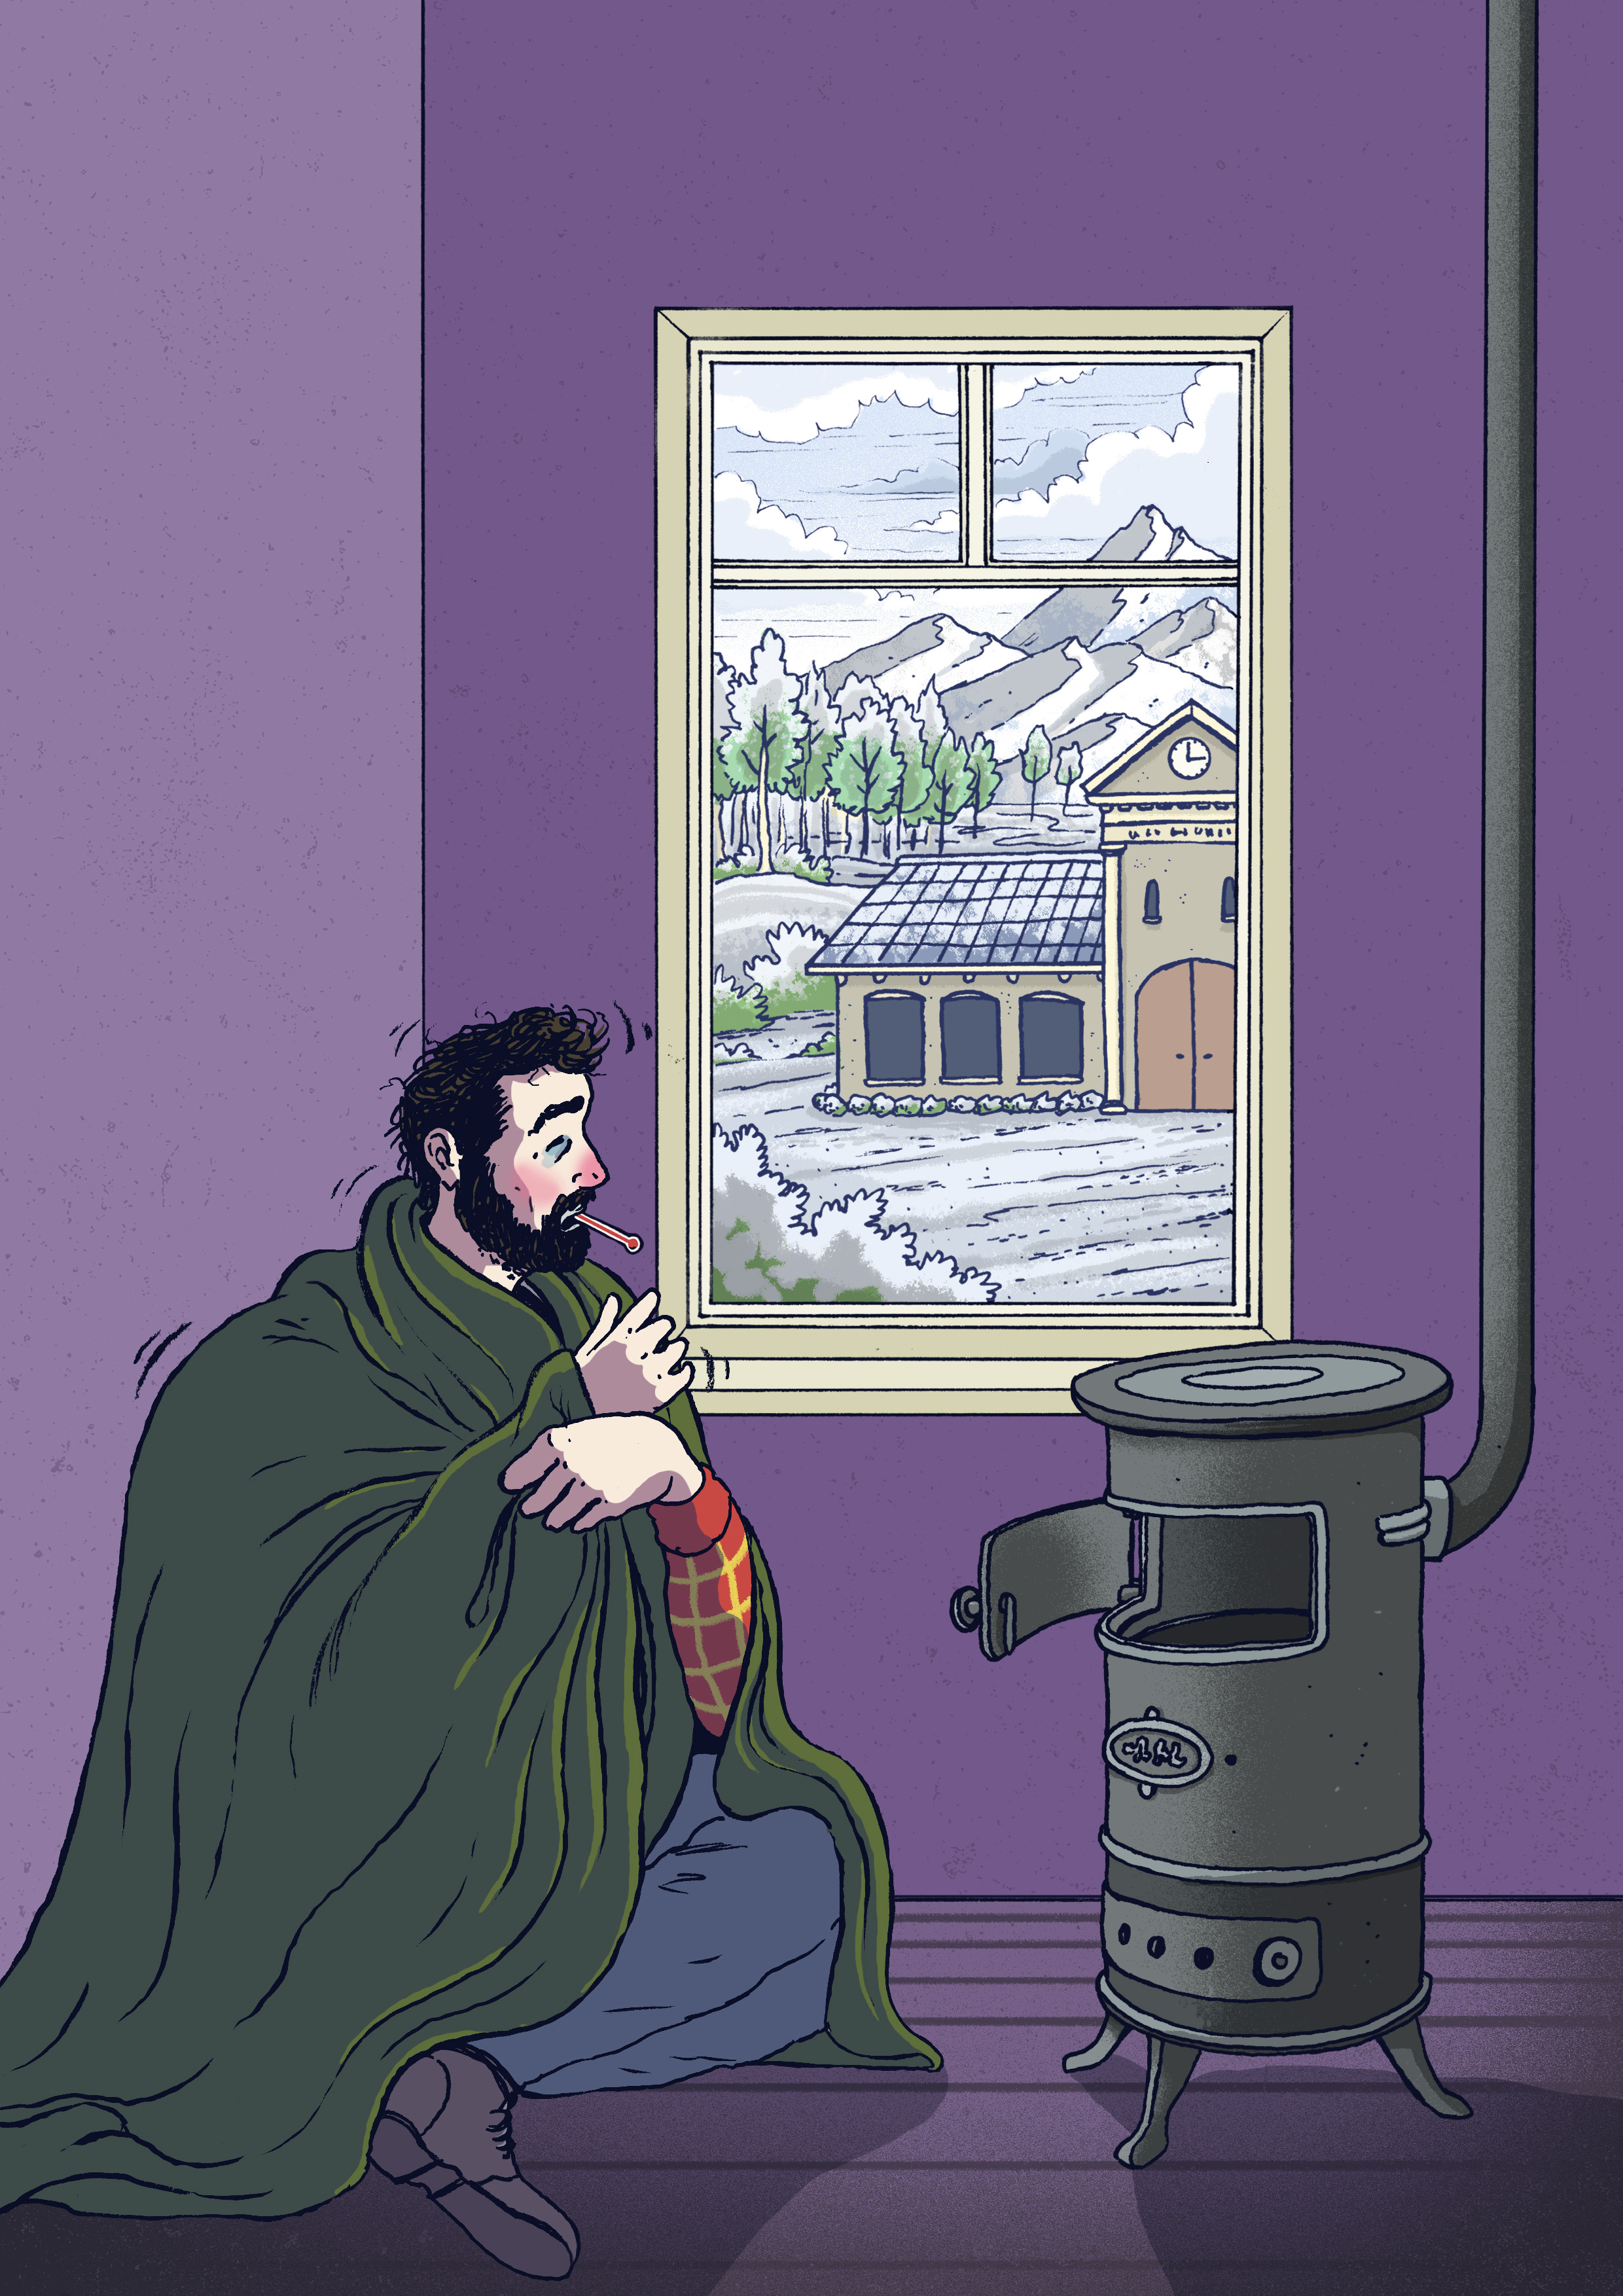
\includegraphics[width=0.8\linewidth]{figures/figure_1_a.jpg}
      \caption{Survival}\label{fig:illu_survival}
   \end{subfigure}
   \hfill
   \begin{subfigure}[t]{0.45\textwidth}
      \centering
      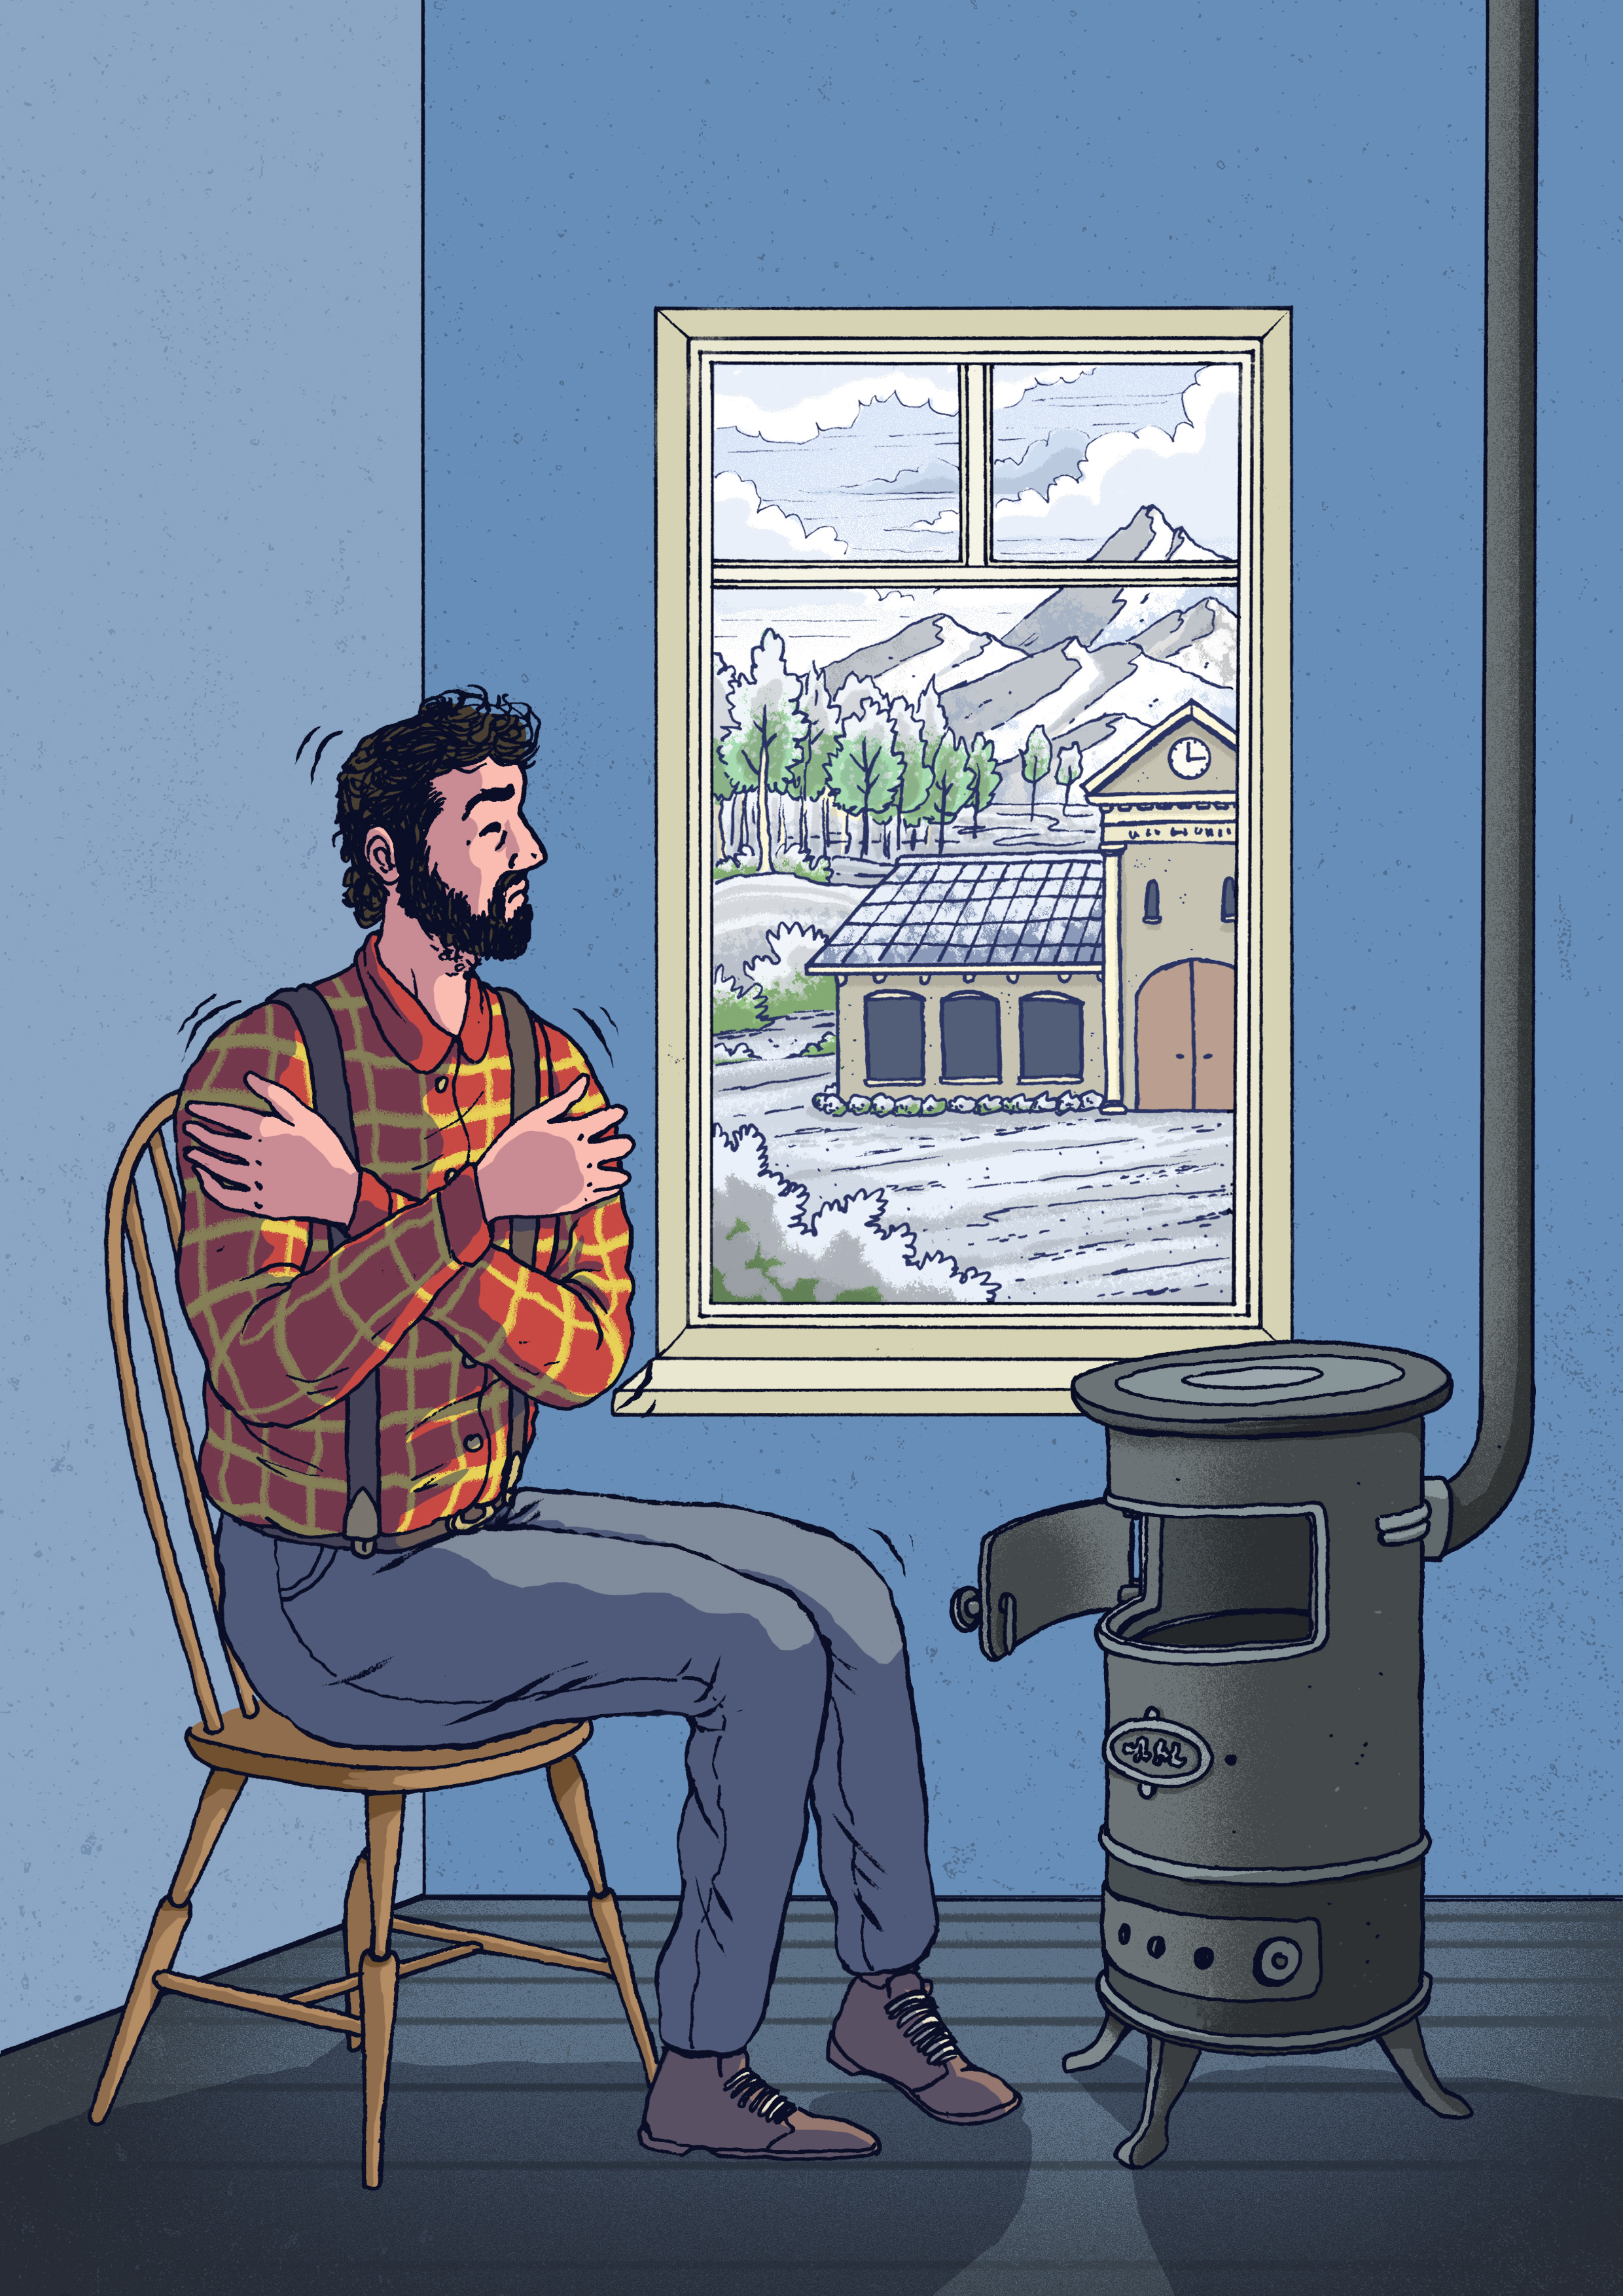
\includegraphics[width=0.8\linewidth]{figures/figure_1_b.jpg}
      \caption{Decency}\label{fig:illu_decency}
   \end{subfigure}
   \begin{subfigure}[t]{0.45\textwidth}
      \centering
      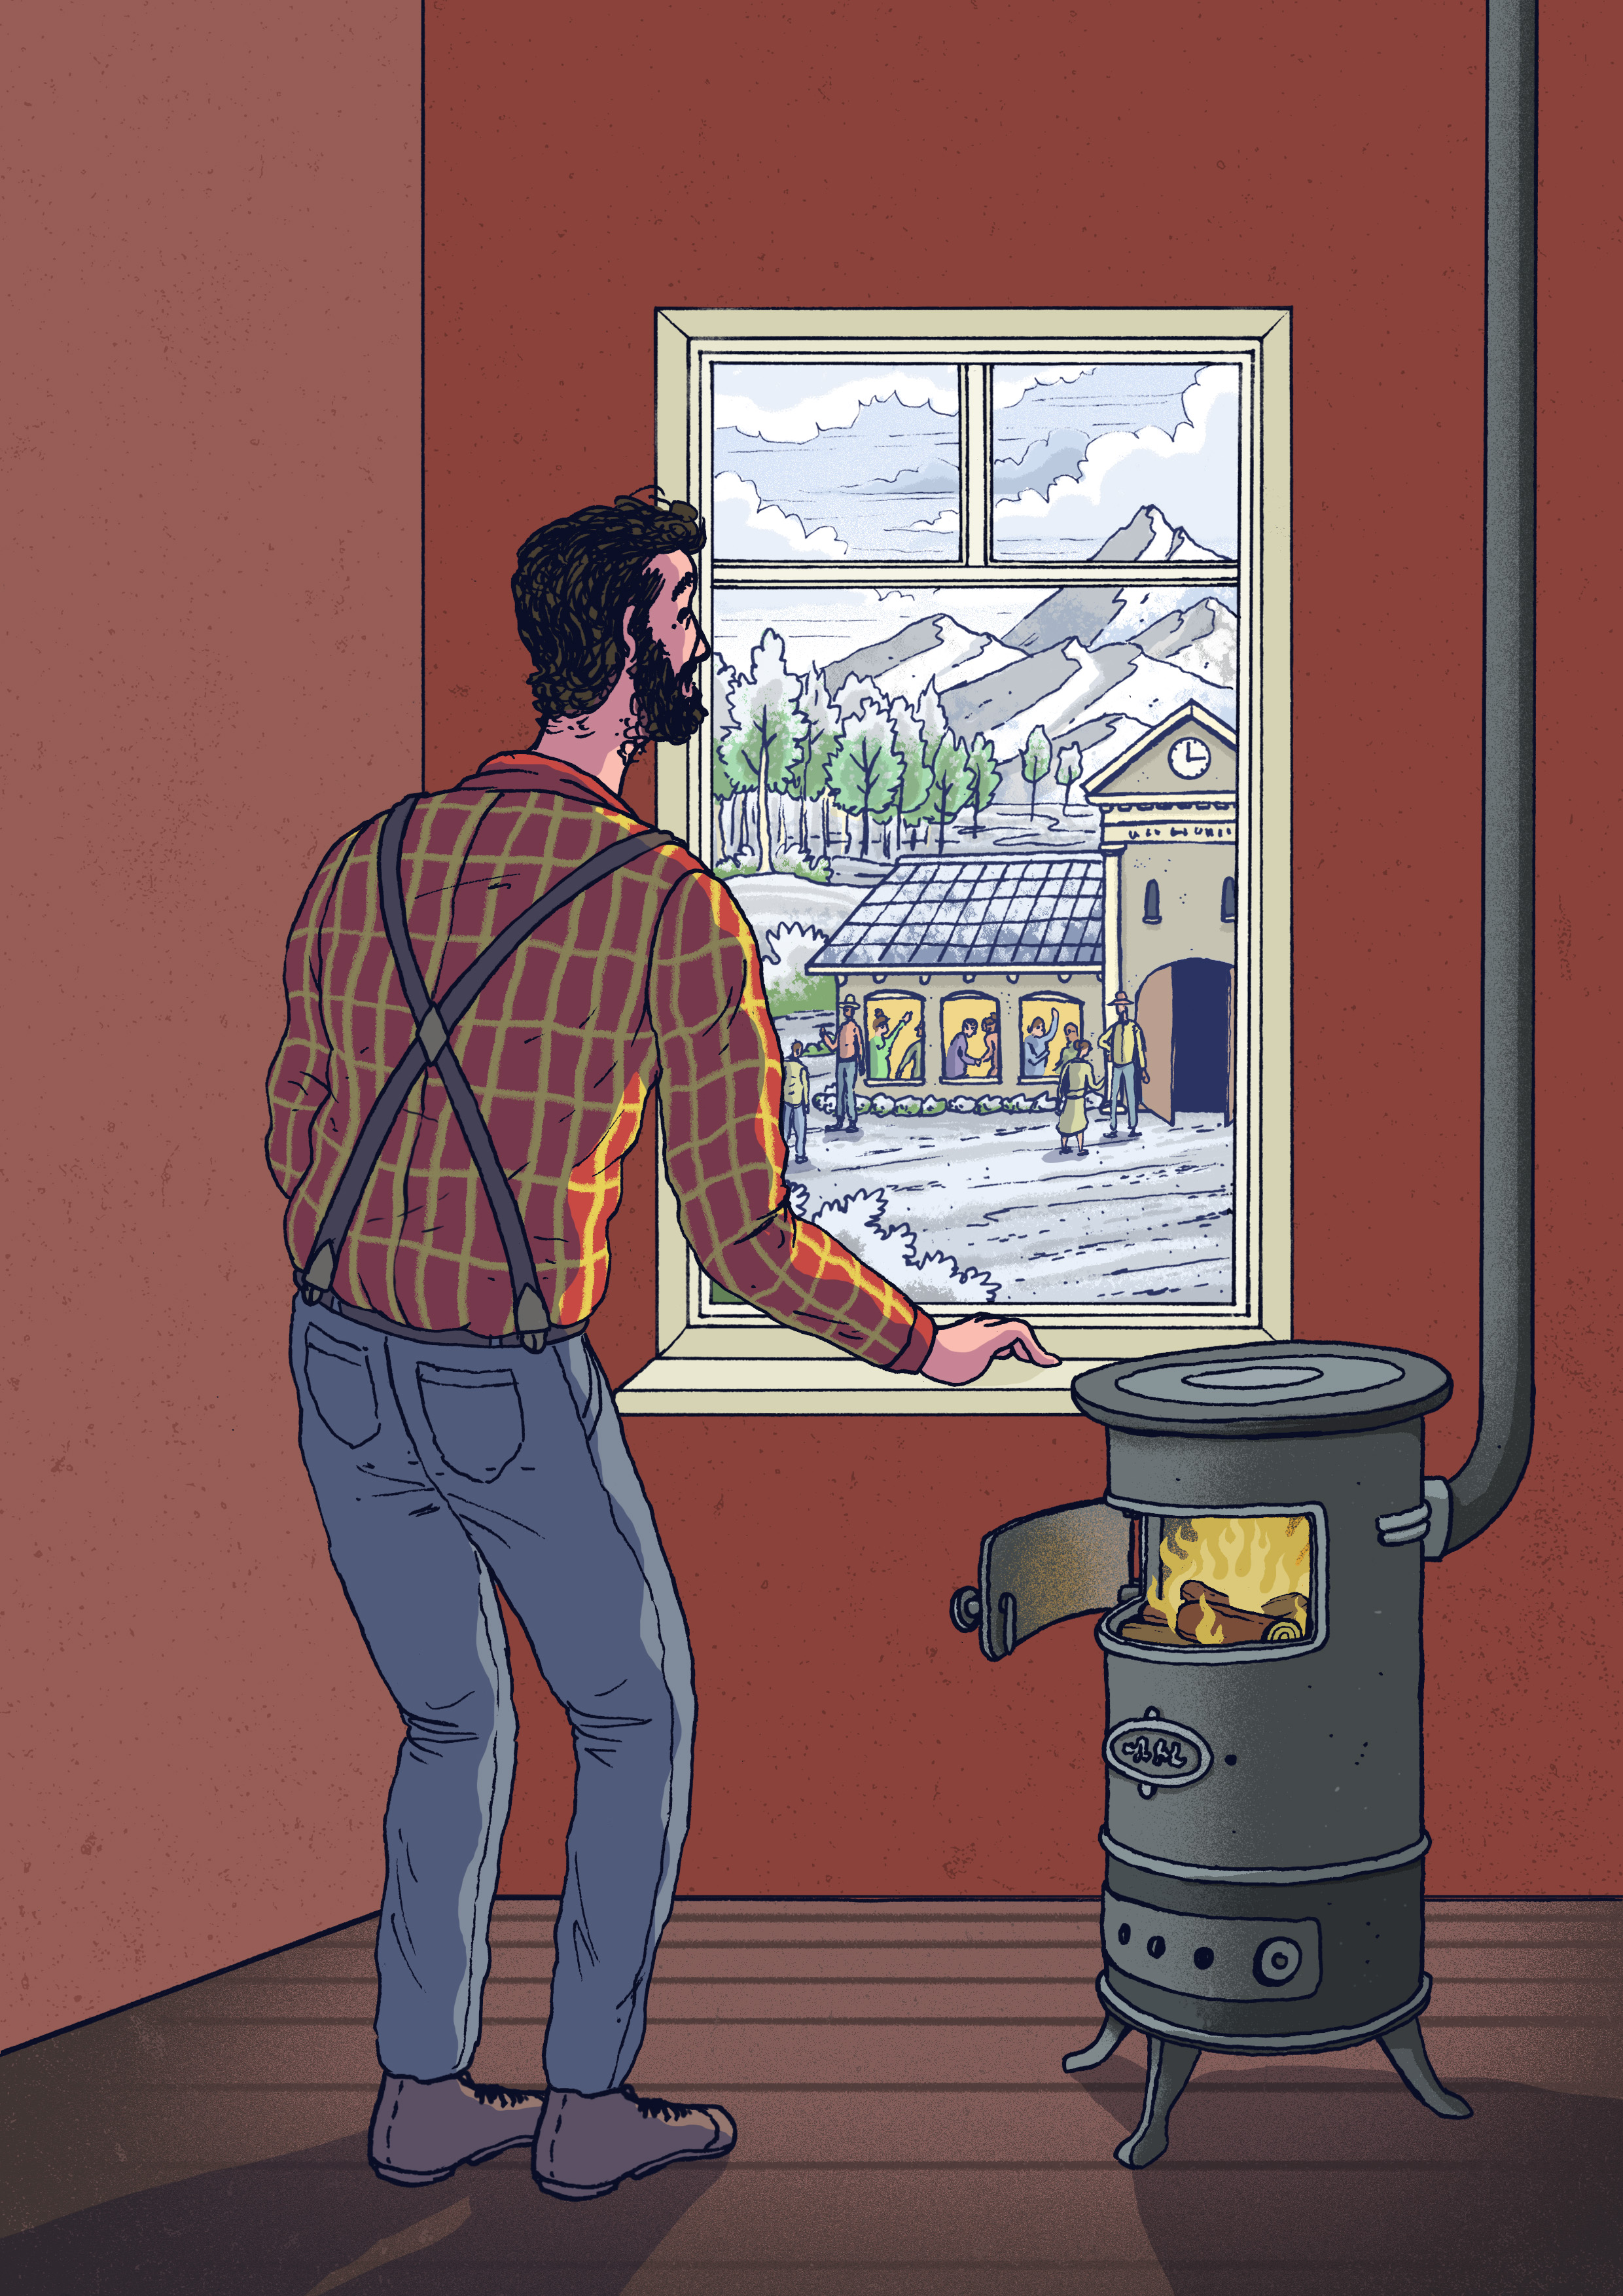
\includegraphics[width=0.8\linewidth]{figures/figure_1_c.jpg}
      \caption{Belonging}\label{fig:illu_belonging}
   \end{subfigure}
   \hfill
   \begin{subfigure}[t]{0.45\textwidth}
      \centering
      
\includegraphics[width=0.8\linewidth]{figures/figure_1_d.jpg}
      \caption{Autonomy}\label{fig:illu_autonomy}
   \end{subfigure}
   \caption{Illustrations presented to participants. Figure \ref{fig:illu_survival} shows the Survival Need, Figure \ref{fig:illu_decency} the Decency Need, Figure \ref{fig:illu_belonging} the Belonging Need, and Figure \ref{fig:illu_autonomy} the Autonomy Need.}\label{fig:illu}
\end{figure}

Following this introduction, the kinds of needs are presented to participants on four separate screens.
Here, they are shown the full-sized illustration with a single caption beneath it describing the kind of need once again as follows:

\begin{itemize}
   \item \textbf{Survival:} ``$A$ needs the wood to make sure to survive the upcoming winter.''
   \item \textbf{Decency:} ``$B$ needs the wood in order not to freeze in the upcoming winter.''
   \item \textbf{Belonging:} ``$C$ needs the wood to be able to participate regularly in the social life of his community in the upcoming winter.''
   \item \textbf{Autonomy:} ``$D$ needs the wood to be able to use his studio regularly in the upcoming winter''.
\end{itemize}

On top of each screen, they are told that they will have to indicate how important they deem the kind of need shown on the page.
On the bottom, they are asked how much the person needs the wood in the present case.
They have to give their answer on a Likert scale from 1 (``doesn't need the wood at all'') to 7 (``absolutely needs the wood'') (see Appendix \ref{sec:app_study_1_instructions} for the instructions of Study 1).
That is, participants indicate how important they consider the satisfaction of the abstract need through a concrete material good. Their evaluation is thus conditional on the situation and the material good.

\subsection{Procedure}\label{sec:study_1_procedure}
The study was programmed in oTree (\citealt{chen_otree_2016}) and ran online in February 2021 with a sample size of $n = 100$.
Participants were recruited by the professional market research institute respondi for a fee, where they were randomly sampled from respondi's online access panel, stratified by the three characteristics gender, age, and equivalent household net income (see Table \ref{tab:quota_study_1} in Appendix \ref{sec:app_additional_tables}).
The data provider has subjected itself to strict ethical guidelines and is certified according to ISO 20252.
Participants must actively opt into the panel and then take part in specific surveys voluntarily.
Since our study is an anonymous standard survey that only uses hypothetical vignettes and assesses uncritical opinions, no additional approval was sought from the ethics commission.
As suggested, e.\,g., by the United States' \textit{Federal Policy for the Protection of Human Subjects}, to ensure informed consent, participants were told at the beginning of each study that the survey at hand is part of a research project, that taking part is voluntary, and that they can drop out at any time.
They were notified how long the survey would approximately take and that its purpose is to assess personal opinions and judgments.
They were also informed that their answers will be analyzed and that all data will be stored in an anonymous format so that no participant can be identified (see Appendix \ref{sec:app_study_1_instructions} and \ref{sec:app_study_2_instructions}.
They were informed beforehand about their compensation by the panel provider.

At the beginning of the study, they were greeted with a welcome message (see Appendix \ref{sec:app_study_1_instructions}).
Thereafter, participants had to evaluate the four kinds of needs as described in Section \ref{sec:study_1_design} (within-participants design).
After this task, three control questions were asked to ensure that participants read the vignettes and instructions carefully (see Appendix \ref{sec:app_study_1_questions}).
As has been announced beforehand, only those participants who passed at least two of our control questions were compensated and included in our analysis.
Failing more than one questions led to an immediate termination of the survey.
Those participants did not receive any further questions.
The 100 participants who answered two or three questions correctly were given a sociodemographic questionnaire asking for their age, gender, household net income, political orientation, and sensitivity to cold (see Appendix \ref{sec:app_study_1_additional_questions}).
They were paid a flat fee of 4.15 euros for approximately 15 minutes of their time.
Another 31 participants were excluded from the study after failing to pass control questions.\footnote{Failure rates indicate that our first question was failed more often than the second and third question (Question 1: 41 of 131 ($31.30\%$), Question 2: 36 of 131 ($27.48\%$), Question 3: 27 of 131 $20.61\%$).
Using $\chi^2$ tests, we found that the excluded participants did not diverge from the remaining participants with regard to age and income at a significance level of $5\%$.
There is, however, a significant difference (at the $1\%$ level) between men and women when it comes to failure rates (Age: $\chi^2=3.787$, $p=0.436$, Income: $\chi^2=8.511$, $p=0.075$), Gender: $\chi^2=7.238$, $p=0.007$).}


\subsection{Working Hypothesis}\label{sec:study_1_hypothesis}
In light of the theoretical literature reviewed in Section \ref{sec:literature}, we suspect that participants ascribe some importance to all four kinds of needs.
We also suspect that the importance of those kinds of needs that are more basic in theory is evaluated higher on average than the importance of those kinds of needs that are less basic in theory.
More specifically, in line with psychological Motivation Theory (\citealt{maslow_theory_1943}, \citealt{alderfer_empirical_1969}) and philosophical considerations (\citealt{braybrooke_meeting_1987}, \citealt{wiggins_needs_1987,wiggins_what_1998}), we hypothesize that physiological needs (survival, decency) receive higher importance ratings than social needs (belonging) and individual needs (autonomy).
If we look at the means ($M$) of importance ratings, we can state as \textbf{Hypothesis 1 (Hierarchy in $M$)}:

\begin{equation}
   M_{Survival} > M_{Decency} > M_{Belonging} > M_{Autonomy}.
\end{equation}


\subsection{Results}
As hypothesized, the importance of the four kinds of needs was rated quite different, as can be seen Figure \ref{fig:study_1_bar}.
The Survival Need scored highest with a mean rating of 6.830 ($\sigma=0.065$, 95\% CI [6.701, 6.959]), followed by the Decency Need with a mean rating of 5.990 ($\sigma=0.098$, 95\% CI [5.796, 6.184]).
Third in line, after a notable drop, is the Belonging Need with a mean rating of 4.051 ($\sigma=0.155$, 95\% CI [3.743, 4.358]), followed by the Autonomy Need with a mean rating of 3.300 ($\sigma=0.160$, 95\% CI [2.982, 3.618]).\footnote{Note that the scale is limited to the interval [1,7]. One could assume that many participants choose the maximum value for Survival, and rightfully so, as 92 of 100 participants did. For Decency, only 31 did so. This in mind, we performed a number of Wilcoxon signed-rank tests to test for differences between the kinds of needs (Survival vs. Decency: $z = 7.348$, $p \leq 0.001$; Decency vs. Belonging: $z = 8.242$, $p \leq 0.001$; Belonging vs. Autonomy: $z = 4.379$, $p \leq 0.001$).}

\begin{figure}[t]
   \centering
   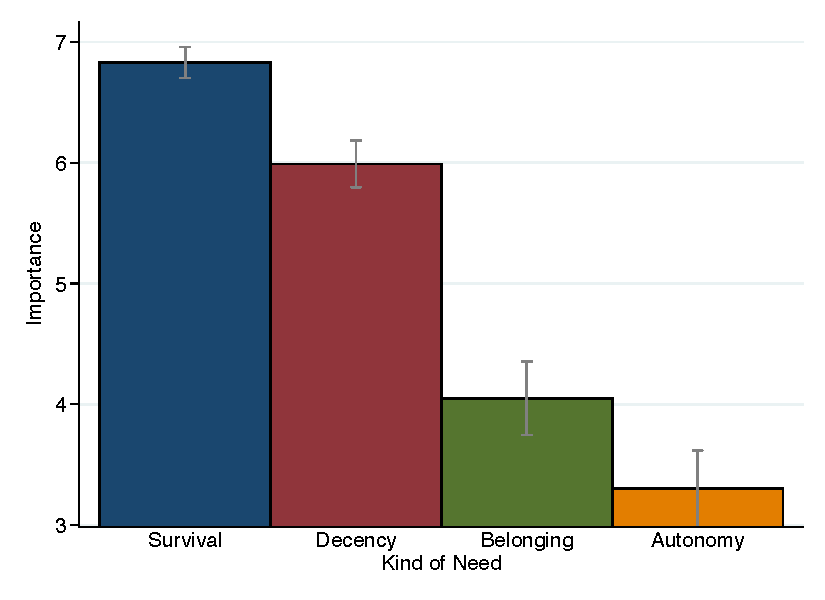
\includegraphics[width=.75\linewidth]{figures/figure_2.pdf}
   \begin{minipage}{0.75\linewidth}
   \footnotesize
   \emph{The figure shows the mean importance ascribed to the four kinds of needs on a scale from 1 (``does not need the wood at all'') to 7 (``absolutely needs the wood''). $n=100$.}
   \end{minipage}
   \caption{Mean importance ascribed to the four kinds of needs}
   \label{fig:study_1_bar}
\end{figure}

As a one-way analysis of variance further shows, pairwise comparisons of all kinds of needs are significant at the $p \le 0.001$ level (see Table \ref{tab:study_1_anova}).
In addition, a pooled OLS regression showed that none of our control variables (age, gender, household net income, political orientation, sensitivity to cold) had a significant effect on our participants' assessments (see Table \ref{tab:reg_study_1} in Appendix \ref{sec:app_additional_tables}).
Here, we clearly see that participants do differentiate when it comes to the importance they ascribe to the different kinds of needs.
Additionally, Table \ref{tab:con_study_1} in Appendix \ref{sec:app_additional_tables} reports contrasts of predictive margins.
Since we used a within-participants design, the individual importance ratings for the four kinds of needs are not independent.
Furthermore, the importance ratings are censored from below (1) and above (7).
Hence, as additional robustness checks, Table \ref{tab:reg_study_1} also includes random-effects panel regressions and Tobit panel regressions.
These lead to qualitatively identical results.

\begin{table}[ht!]
   \centering
   \caption{Mean importance ascribed to kinds of needs and differences between them}\label{tab:study_1_anova}
   \begin{tabular}{lcccc}\\[0.5ex]
   \hline
                & Survival         & Decency          & Belonging        & Autonomy   \\
   \hline
   Mean         & $ 6.830$         & $ 5.990$         & $ 4.051$         & $3.300$    \\
   Std. Dev.    & $ 0.065$         & $ 0.098$         & $ 0.155$         & $0.160$    \\
   \hline\hline
   Decency      & $-0.840^{***}$   &                  &                  &            \\
   Belonging    & $-2.779^{***}$   & $-1.939^{***}$   &                  &            \\
   Autonomy     & $-3.530^{***}$   & $-2.690^{***}$   & $-0.751^{***}$   &            \\
   \hline
   \multicolumn{5}{p{10.5cm}}{\footnotesize{\textit{Upper panel: Mean of the ascribed importance and Standard Deviation. Lower panel: Mean differences. $n=100$. Significance levels: * p $\le$ 0.1, ** p $\le$ 0.05, *** p $\le$ 0.001, Bonferroni adjusted.}}}
   \end{tabular}
\end{table}


%%%%%%%%%%%
% STUDY 2 %
%%%%%%%%%%%
\section{Study 2}\label{sec:study_2}
\subsection{Design}
For our second study, we join the vignette of Study 1 with a vignette by \cite{bauer_need_2022}.
In \cite{bauer_need_2022}, participants are asked to imagine two hypothetical persons.
Their names are drawn randomly from a list of common German surnames.
In the following, we simply refer to them as ``Person A'' and ``Person B''.
Person A and Person B are both in need for firewood.
Their community allows them to chop wood in the community's forest for a certain period of time, which is the only way for Person A and Person B to get firewood, since both have little money.

In the fashion of Study 1, we alter the vignette by adding the four different kinds of needs that Person A and Person B can experience (see Section \ref{sec:study_1_design}).
Participants are introduced to those four kinds at the study's beginning.
As in Study 1, each vignette (see Appendix \ref{sec:app_study_2_instructions} for wordings) is presented next to a picture that illustrates the kind of need in question (see Figure \ref{fig:illu} again).

Subsequent to this introduction, participants are introduced to their task, which is to distribute an endogenously given number of logs---described as the total amount of wood both have chopped---among Person A and Person B in a way participants think to be most just.
They are made aware that in doing so they will have to make trade-offs between Person A and Person B; the more wood they give to one person, the less they can give to the other.
Still more, we revealed that it would not be possible to completely meet the needs of both persons at the same time, as the available amount of wood was just about enough to completely cover the needs of one of the two persons; the other person would then end up empty-handed.
In case a person receives less wood than they need, the person will suffer certain consequences, depending on the kind of need they experience.
Participants were further informed that they would distribute the wood in advance without knowing exactly how cold the winter actually will be.
This is why we describe the possible effects of the upcoming winter on the respective person as ``more or less likely''.

\begin{figure}[t]
   \centering
   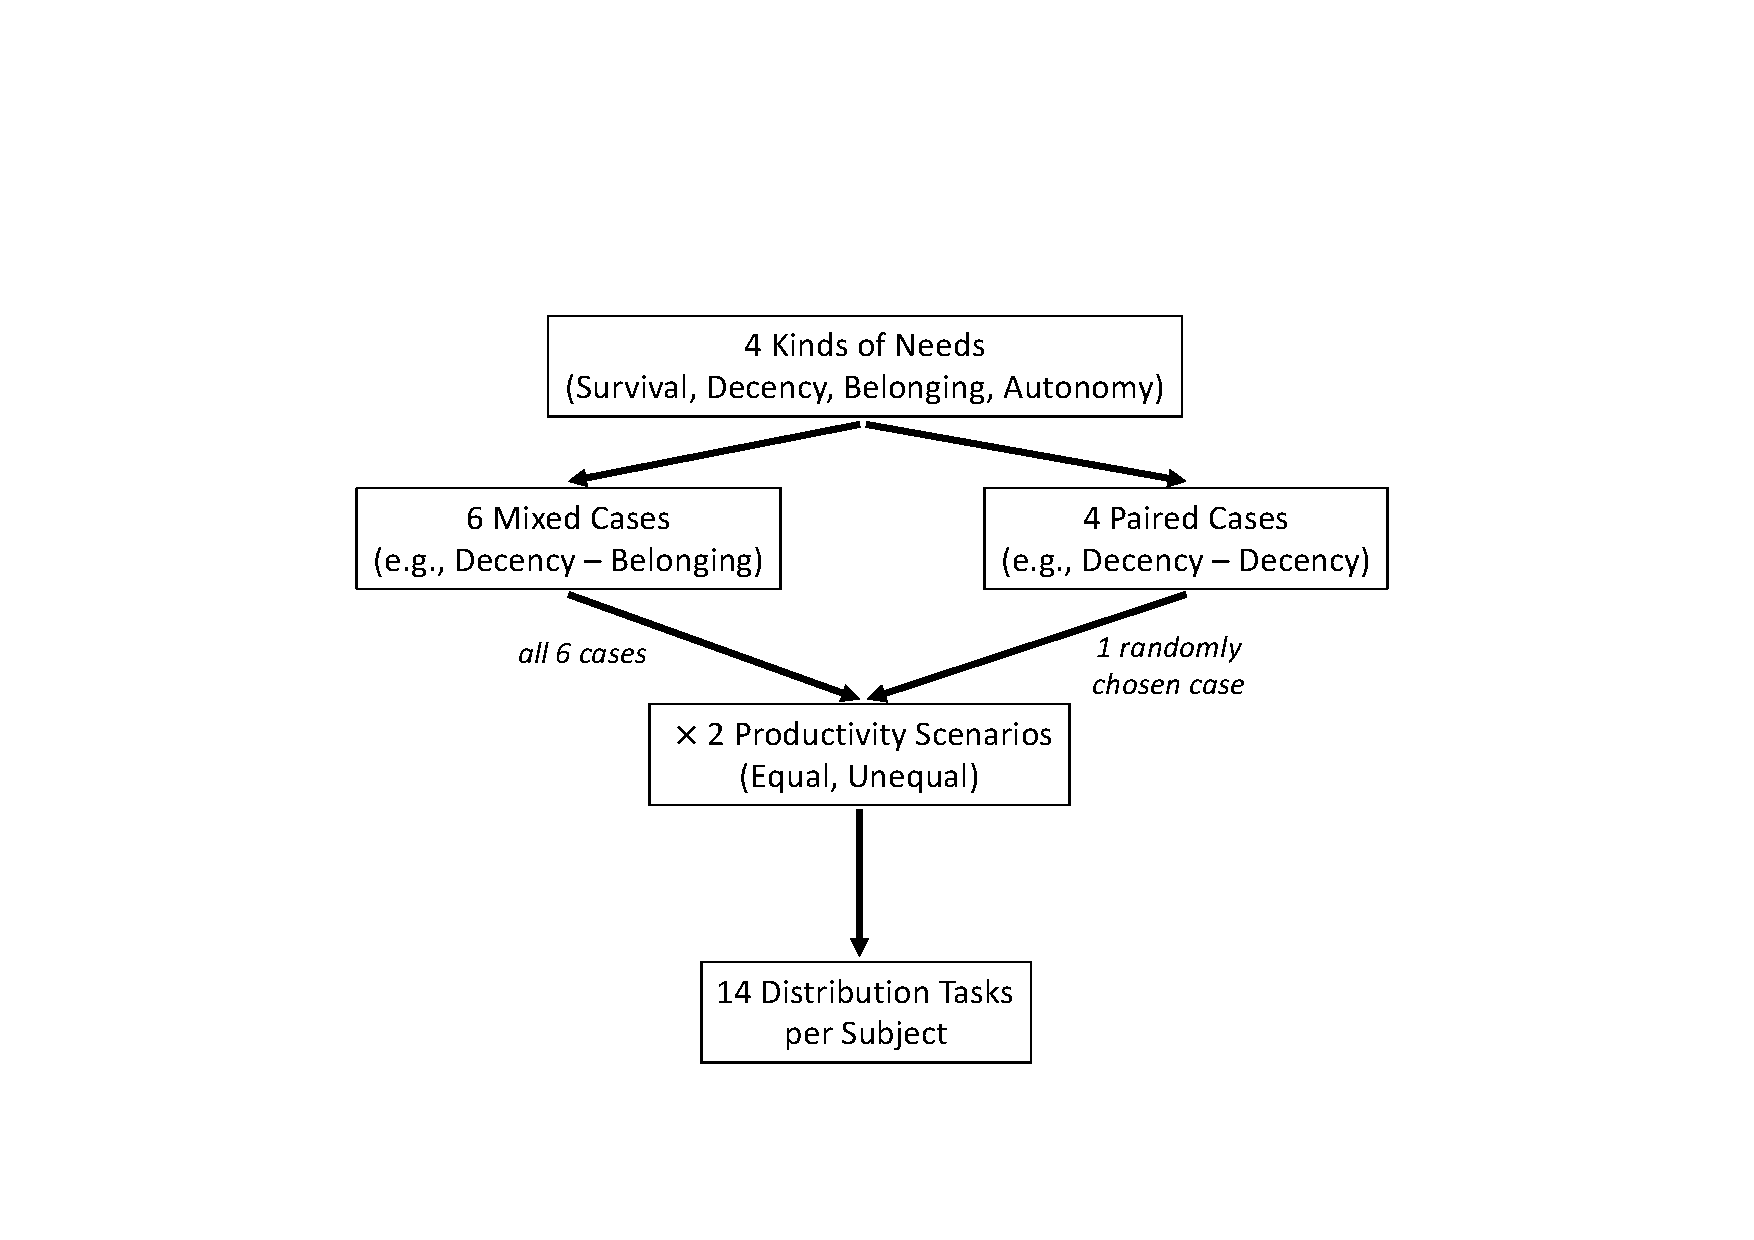
\includegraphics[width=1\linewidth]{figures/figure_3.pdf}
   \caption{Within-participants variations of Study 2}
   \label{fig:study_2_design}
\end{figure}

The design of Study 2 is schematized in Figure \ref{fig:study_2_design}.
As can be seen there, each participant had to make a total of 14 different allocation decisions, denoted as \textit{Cases} in the following.
For each case, they had to decide how much wood to give to Person A and Person B.
Those 14 cases were split into two different \textit{Scenarios} with 7 cases each.
This within-participants variation altered whether Person A and B have chopped the same amount or different amounts of wood.
In the \textit{Equal Productivity Scenario}, Person A and Person B have chopped 500 logs each, in the \textit{Unequal Productivity Scenario}, Person A has only chopped 200 logs, while Person B has chopped 800 logs.
Note that the total amount of logs is constant over every case and over both scenarios.
We randomized whether participants started with the Equal Productivity Scenario or the Unequal Productivity Scenario.
Within each Scenario, we further randomized the order of appearance of the seven cases.

The seven cases themselves vary what Person A and Person B need the wood for (i.\,e., which kind of need they experience).
Here, we distinguish between \textit{Mixed Cases} and \textit{Paired Cases}.
In Mixed Cases Person A and Person B experience two different kinds of needs, whereas in Paired Cases they experience the same kind of need.
While Paired Cases give us a baseline and a consistency check, mixed cases provide us with the differences between the kinds of needs that are in our focus.
Six of the seven cases a participant sees per scenario are \textit{Mixed Cases}, containing the possible combinations that can be obtained from the four different kinds of needs without creating pairs, as depicted in Table \ref{tab:combinations}.
One additional case a participant sees per scenario is---randomly drawn---\textit{one} of the four possible \textit{Paired Cases}, which shows the same pair in both scenarios.

\begin{table}[ht!]
   \centering
   \caption{Combinations made from Kinds of Needs for each Case of a Scenario}\label{tab:combinations}
   \begin{tabular}{ccccccc}\hline
               & \multicolumn{6}{c}{Case}                                                       \\\cline{2-7}
      Person   & 1          & 2           & 3          & 4           & 5          & 6           \\\hline\hline
      A        & Survival   & Survival    & Survival   & Decency     & Decency    & Belonging   \\
      B        & Decency    & Belonging   & Autonomy   & Belonging   & Autonomy   & Autonomy    \\\hline
   \multicolumn{7}{p{14.2cm}}{\footnotesize{\textit{The combinations made from the four Kinds of Needs for the six Mixed Cases of each Scenario.}}}
   \end{tabular}
\end{table}

Between-participants, we implement two different \textit{Formulations} in which we present those descriptions of the different kinds of needs and their consequences either as the avoidance of negative consequences (\textit{Avoidance Formulation}) or as the enablement of good outcomes (\textit{Enablement Formulation}) to check whether possible effects are influenced by the way we present the kinds of needs.

Each case is presented on a separate screen (see the exemplary task in Appendix \ref{sec:app_study_2_instructions} for an example).
On every screen, we randomize the position of Person A and Person B.
Participants are informed how much wood Person A and Person B have chopped each and in total on each screen.
In the center of every screen, two illustrations are displayed side by side to highlight the kind of need Person A and Person B exhibit in the displayed case.
Below each picture, a single sentence additionally makes clear what Person A and Person B need the wood for:

\begin{itemize}
   \item \textbf{Survival:} ``$A$ $[B]$ needs the wood to avoid life-threatening illness [stay healthy] in the upcoming winter.''
   \item \textbf{Decency:} ``$A$ $[B]$ needs the wood to avoid freezing [have it warm] in the upcoming winter.''
   \item \textbf{Belonging:} ``$A$ $[B]$ needs the wood in order not to be excluded from [to participate in] social life in the upcoming winter.''
   \item \textbf{Autonomy:} ``$A$ $[B]$ needs the wood so that their studio does not become unusable [so that they can use their studio] in the upcoming winter.''
\end{itemize}

Participants are asked to enter the amount Person A and Person B should receive on a blank line in a sentence below each picture that stated ``$A$ $[B]$ should receive \_\_\_ logs of wood''.
Here, all available logs have to be distributed by them.

Mixed Cases, Paired Cases, and Productivity Scenarios are varied within-participants because otherwise only the treatment mean differences and not the mean values of the individual differences could be analyzed.
Formulations are varied between-participants to keep the number of cases that are presented to participants manageable, hence to avoid fatigue effects, and to prevent contrast effects, which would make it difficult to find out if the wording actually makes a difference.


\subsection{Procedure}
Our study, programmed in oTree \citep{chen_otree_2016}, was conducted online in April 2021.
The total sample size was $n = 200$.
Participants were recruited via the private market research institute respondi, being randomly sampled from respondi's online access panel, stratified by the characteristics gender, age, and household net income to promote external validity (see Table \ref{tab:quota_study_2} in Appendix \ref{sec:app_additional_tables}).
Sampling rates of these characteristics have been taken from the ``Best for Planning'' study of Germany's \textit{Society for Integrated Communication Research} as representative for the adult German population (\citealt[p. 284, 291]{gesellschaft_fur_integrierte_kommunikationsforschung_best_2019}).

To control for the heterogeneity of our participants with regard to their sociodemographic backgrounds and justice attitudes, we implemented a questionnaire, where we asked participants for their age, gender, and household net income.
Furthermore, they had to state their support for the three different distributive principles of need, equity, and equality, as well as their political orientation, all on 7-point Likert scales.
Lastly, they were asked how they perceive their own sensitivity to cold (see Appendix \ref{sec:app_study_2_additional_questions} for wordings).

To facilitate internal validity and to ensure that our vignettes and instructions were read thoroughly, participants had to answer three control questions after they completed the distribution task (see Appendix \ref{sec:app_study_2_control_questions} for wordings).
The final analysis was restricted to those participants who passed at least two of the three questions.
Those 200 participants were paid a flat fee of 5.40 euros, being equivalent to an hourly wage of 10.80 euros.
64 participants were excluded since they failed to pass at least two of our three control questions.
For them, the survey was terminated after giving two wrong answers and they were asked no further questions.\footnote{Failure rates indicate that our second question was failed more often than the first and third question (Question 1: 83 of 264 ($31.44\%$), Question 2: 119 of 264 ($45.08\%$), Question 3: 68 of 264 ($25.76\%$), see Appendix \ref{sec:app_study_2_control_questions} for the questions' wording).
Excluded participants did not diverge from the remaining participants in age, income, or gender at a significance level of $5\%$ (Age: $\chi^2=2.049$, $p=0.727$, Income: $\chi^2=1.657$, $p=0.799$, Gender: $\chi^2=0.047$, $p=0.828$).}


\subsection{Working Hypotheses}
A little notation first.
Let $\mathcal{I}=\{1,2,\ldots,n\}$ denote the set of participants $i$ and $\mathcal{N}=\{1\ (\text{Survival}), 2\ (\text{Decency}), 3\ (\text{Belonging}), 4\ (\text{Autonomy})\}$ the ordered set of the kinds of needs $\alpha, \beta$.
Needs are ordered in terms of decreasing priority as elicited in Study 1, i.\,e., $\alpha<\beta$.
In the relative evaluation task, participant $i$ is endowed with $\ell^i=1000$ logs of wood.
They assign $0 > \ell^i_\alpha\le 1000$ logs to Person A with need $\alpha$ and $\ell^i_\beta=1000-\ell^i_\alpha$ logs to Person B with need $\beta$.
The relative evaluation of Person A's need $\alpha$ by participant $i$ is hence given by $\Delta^i_{\alpha,\beta}=\ell^i_\alpha-\ell^i_\beta=2\ell^i_\alpha-1000$.

We start with the Equal Productivity Scenario (EPS).
For \textit{paired} need evaluations $\alpha=\beta$, we expect the mean relative need evaluation to be zero: $\overline{\Delta}^\text{EPS}_{\alpha,\alpha}=0$.
For \textit{mixed} need evaluations $\alpha<\beta$, we expect the mean relative need evaluation to increase in the distance between absolute need evaluations.
Hence, \textbf{Hypothesis 2 (Hierarchy in $\Delta$)} reads as follows:

\begin{equation}
   \overline{\Delta}^\text{EPS}_{\alpha,\beta}>\overline{\Delta}^\text{EPS}_{\alpha,\beta'},\quad\beta>\beta'.
\end{equation}

\noindent We further assume that participants make coherent distributive decisions.
A decision is coherent if the differences we observe in mean allocations are additive.
In other words, it is coherent if the difference of two kinds of needs, being not next to each other in the hierarchy, equals the sum of the differences of the kinds of needs that are spanned by the original difference.
Hence, \textbf{Hypothesis 3 (Coherence)} states:

\begin{equation}
   \overline{\Delta}^\text{EPS}_{\alpha,\beta}=\overline{\Delta}^\text{EPS}_{\alpha,\beta'}+\overline{\Delta}^\text{EPS}_{\beta',\beta''}+\overline{\Delta}^\text{EPS}_{\beta'',\beta},\quad\alpha\le\beta'\le\beta''\le\beta.
\end{equation}

\noindent In the Unequal Productivity Scenario (UPS), the relative need evaluation for pairs $\alpha=\beta$ does not need to be zero if productivity matters.
In fact, we expect the need evaluation to be lower for the less productive Person A: $\overline{\Delta}^\text{UPS}_{\alpha,\alpha}<0$.
However, we expect the impact of lower productivity on relative need evaluations to decrease with the importance of need: $\overline{\Delta}^\text{UPS}_{\alpha,\alpha}-\overline{\Delta}^\text{UPS}_{\alpha',\alpha'}>0$ for $\alpha<\alpha'$.
For mixed need evaluations, as in EPS, we expect mean relative need evaluations to increase with the distance between absolute need evaluations.
Hence, \textbf{Hypothesis 4 (Productivity)} ready as follows:

\begin{equation}
   \overline{\Delta}^\text{UPS}_{\alpha,\beta}>\overline{\Delta}^\text{UPS}_{\alpha,\beta'},\quad\beta>\beta'.
\end{equation}

\noindent Here, we also expect relative need evaluations to be coherent $\overline{\Delta}^\text{UPS}_{\alpha,\beta}=\overline{\Delta}^\text{UPS}_{\alpha,\beta'}+\overline{\Delta}^\text{UPS}_{\beta',\beta''}+\overline{\Delta}^\text{UPS}_{\beta'',\beta}$, where $\alpha\le\beta'\le\beta''\le\beta$.


\section{Results}\label{sec:results}
We start with taking a look at the Paired Cases (Section \ref{sec:results_mean_paired}) before moving on to the Mixed Cases (Section \ref{sec:results_mean_mixed}).
After looking at the mean differences, we examine the coherence of our participants' decisions (Section \ref{sec:results_additivity}) and, finally, we present a number of regressions (Section \ref{sec:results_regressions}).


\subsection{Mean Differences in Allocations for Paired Cases}\label{sec:results_mean_paired}
First, we take a look at the relative evaluations, i.\,e., the way participants allocated the logs of firewood between the two persons presented to them.
Since Paired Cases give us a baseline and a consistency check, we start with having a look at them.
To do so, we calculate the mean of the individual differences (represented by $\Delta$) of the number of logs participants gave to Person A and Person B in those four cases (see Table \ref{tab:means_mixed_paired} in Appendix \ref{sec:app_additional_tables}).

Figure \ref{fig:overview_paired} shows the mean differences for the four Paired Cases.
The bars are differentiated by the two Productivity Scenarios that were presented within-participants.
We see that in the Equal Productivity Scenario participants by and large distribute equally between Person A and Person B, resulting in a mean difference of (roughly) around $0$.
Since both persons have contributed the same amount of wood and exhibit the same kind of need, this is, arguably, the only reasonable default, which is a strong indicator that our participants understood the vignette and task and took it seriously.

\begin{figure}[t]
   \centering
   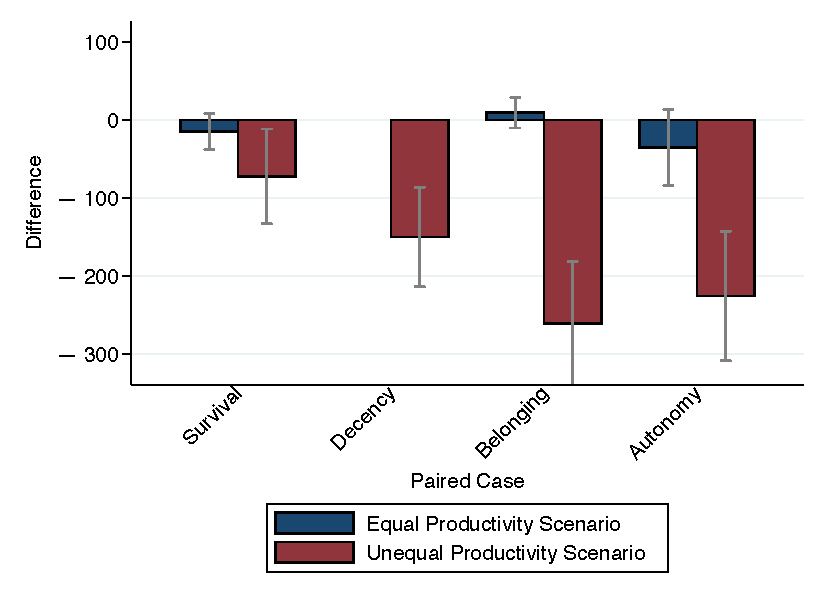
\includegraphics[width=.75\textwidth]{figures/figure_4.pdf}
   \begin{minipage}{0.75\linewidth}
   \footnotesize
   \emph{The figure shows the mean differences in allocations to Person A and Person B, experiencing the same kind of need, by Productivity Scenario. $n = 200$.}
   \end{minipage}
   \caption{Mean differences for the 4 Paired Cases by Productivity Scenario}
   \label{fig:overview_paired}
\end{figure}

However, in the Unequal Productivity Scenario, where Person A has cut 200 logs and Person B 800 logs, Person A gets less than Person B.
Interestingly, this depends on the kind of need as hypothesized above.
If both need the wood for survival, the lower productivity of Person A has hardly any effect, that is, she gets only a little less than Person B although she has cut much less.
The difference is a bit more pronounced for the second kind of need, Decency, and is largest for Belonging and Autonomy.
But even there, Person A still gets significantly more than she has initially contributed.
See also Table \ref{tab:means_deviation_paired} in the Appendix, reporting means of absolute percentage deviations of the share that Person A receives from the share that Person A contributed.

Table \ref{tab:means_deviation_paired} additionally shows by how many percent the share that the needier Person A receives differs from the share of their contribution (normalized to $0-100\%$).
This deviation can be interpreted as a kind of elasticity of need satisfaction for productivity; the larger this deviation, the more important needs are considered.
In the Equal Productivity Scenario, as would be expected, this rambles around roughly 1\%.
In the Unequal Productivity Scenario, on the other hand, we get a benchmark for the marginal effect of productivity for the same kinds of needs.
This is a first measure of the importance of the different kinds of needs, because the more productivity matters, the less the equality of needs matters.
The difference is highest for survival (10.556\%), followed by decency (9\%), autonomy (7.486\%) and belonging (6.791\%).


\subsection{Mean Differences in Allocations for Mixed Cases}\label{sec:results_mean_mixed}
Next, we consider the Mixed Cases.
Again, we calculate the mean of the individual differences of the number of logs participants gave to Person A, experiencing one kind of need, and Person B, this time experiencing another, less basic, kind of need (see Table \ref{tab:means_mixed_paired} in Appendix \ref{sec:app_additional_tables}).

Figure \ref{fig:overview_mixed} presents the mean differences for the six possible combinations that can be made with Person A and Person B experiencing different kinds of needs, again by Productivity Scenario.
It becomes apparent that in the Unequal Productivity Scenario the mean differences are smaller than in the Equal Productivity Scenario for every combination.
In Table \ref{tab:means_mixed_paired}, we additionally report two-tailed Welch's t-tests for the difference between the Productivity Scenarios showing that mean differences for all cases are significantly lower in the Unequal Productivity Scenario.
Differences between Cases are tested in a series of regressions, see Section \ref{sec:results_regressions}.

\begin{figure}[t]
   \centering
   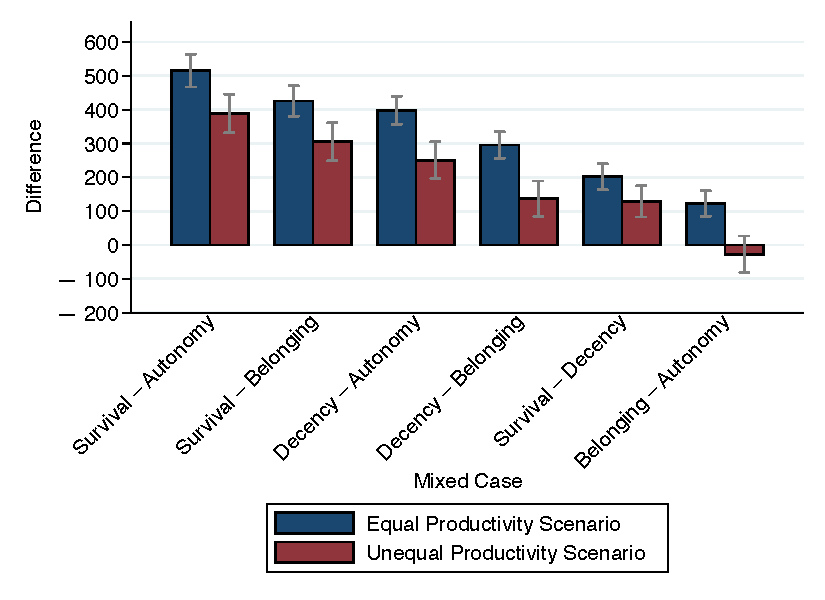
\includegraphics[width=.75\textwidth]{figures/figure_5.pdf}
   \begin{minipage}{0.75\linewidth}
   \footnotesize
   \emph{The figure shows the mean differences in allocations to Person A and Person B, experiencing different kinds of needs, by Productivity Scenario. $n = 200$.}
   \end{minipage}
   \caption{Mean differences for the 6 Mixed Cases by Productivity Scenario}
   \label{fig:overview_mixed}
\end{figure}

Furthermore, if we assume that there is an order of the four kinds of needs, as proposed in Section \ref{sec:literature}, we can see that the differences are larger for those combinations that represent kinds of needs that are not located ``next to each other'' in the hierarchy.
Spanning all four kinds of needs, the difference for the case \textit{Survival -- Decency} is largest, followed by those two cases that span three kinds of needs, namely \textit{Survival -- Belonging} and \textit{Decency -- Autonomy}.
Lastly, those combinations representing kinds of needs that are adjacent to each other, the cases \textit{Survival -- Decency}, \textit{Decency -- Belonging}, and \textit{Belonging -- Autonomy}, show the smallest differences.
These observations can be seen as a hierarchy in the perception of the different kinds of needs that is in line with the theoretical predictions.
The difference for the case \textit{Survival -- Autonomy} is largest, just as those kinds of needs are furthest from each other in theory.
For the cases \textit{Survival -- Belonging} and \textit{Decency -- Autonomy}, the difference is clearly smaller.
Even more so for the cases \textit{Survival -- Decency} and \textit{Belonging -- Autonomy}.
This lends support to our Hierarchy Hypothesis.


\subsection{Additivity of Allocations}\label{sec:results_additivity}
In addition to the hierarchy observed above, we assume that rational people make coherent differentiations when distributing resources among people who experience different kinds of needs.
As has been noted in connection with our Coherence Hypothesis, we speak of coherent differentiations when they are additive.
Additivity is given if the $\Delta$ of two kinds of needs, being not next to each other in the hierarchy, equals the sum of the differences of the kinds of needs that are spanned by the original $\Delta$.

\begin{figure}[t]
   \centering
   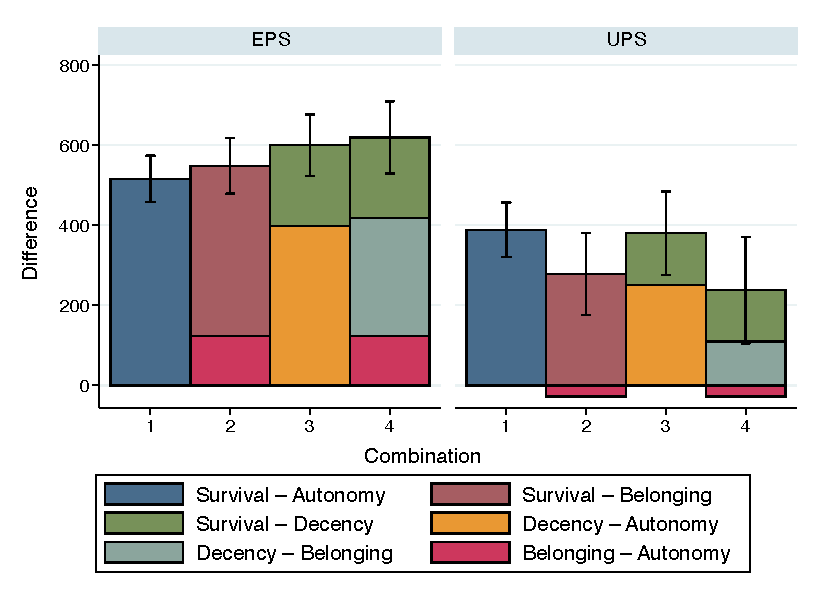
\includegraphics[width=.75\textwidth]{figures/figure_6.pdf}
   \begin{minipage}{0.75\linewidth}
   \footnotesize
   \emph{The figure shows a comparison between the reference case ``Survival -- Autonomy'' and the possible additions by Productivity Scenario. $n = 200$.}
   \end{minipage}	
   \caption{Additivity of importance ratings: Survival -- Autonomy}
   \label{fig:additivity_all}
\end{figure}

Figure \ref{fig:additivity_all} to \ref{fig:additivity_sub_2} indicate that this, indeed, seems to be the case.
In Figure \ref{fig:additivity_all}, the first bar shows the difference of the case \textit{Survival -- Autonomy} as reference, both in the Equal and the Unequal Productivity Scenario.
The following three bars then show the three possible additions, as introduced in Equation (6), above.
In Figure \ref{fig:additivity_sub_1}, the first bar shows the case \textit{Decency -- Autonomy} as reference, again both for the Equal and the Unequal Productivity Scenario, followed by the analogous addition of \textit{Belonging -- Autonomy} and \textit{Decency -- Belonging} in the next bar.
In Figure \ref{fig:additivity_sub_2}, the first bar shows the case of \textit{Survival -- Belonging}, once more for both the Equal and the Unequal Productivity Scenario, followed by the analogous addition of \textit{Decency -- Belonging} and \textit{Survival -- Decency} in the second bar.

\begin{figure}[ht!]
   \centering
   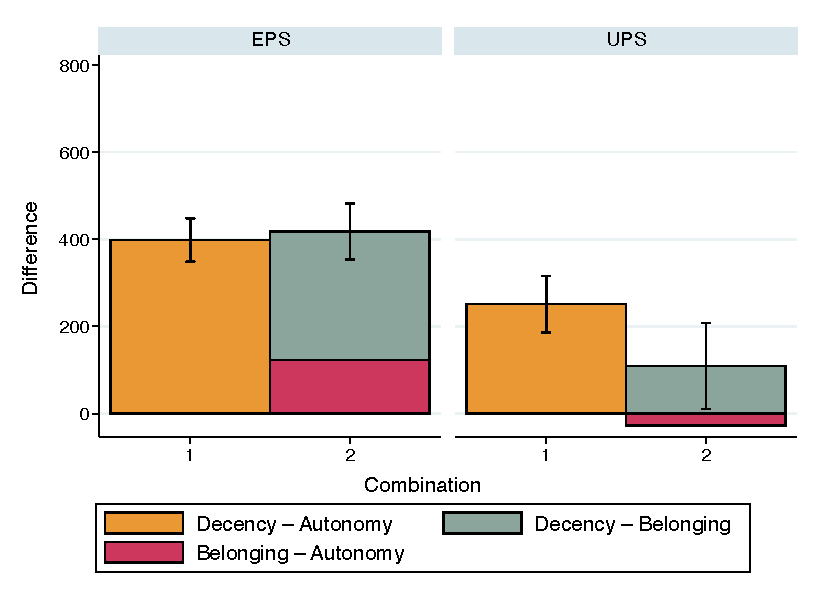
\includegraphics[width=.75\textwidth]{figures/figure_7.pdf}
   \begin{minipage}{0.75\linewidth}
   \footnotesize
   \emph{The figure shows a comparison between the reference case ``Decency -- Autonomy'' and the possible addition by Productivity Scenario. $n = 200$.}
   \end{minipage}	
   \caption{Additivity of importance ratings: Decency -- Autonomy}
   \label{fig:additivity_sub_1}
\end{figure}

\begin{figure}[ht!]
   \centering
   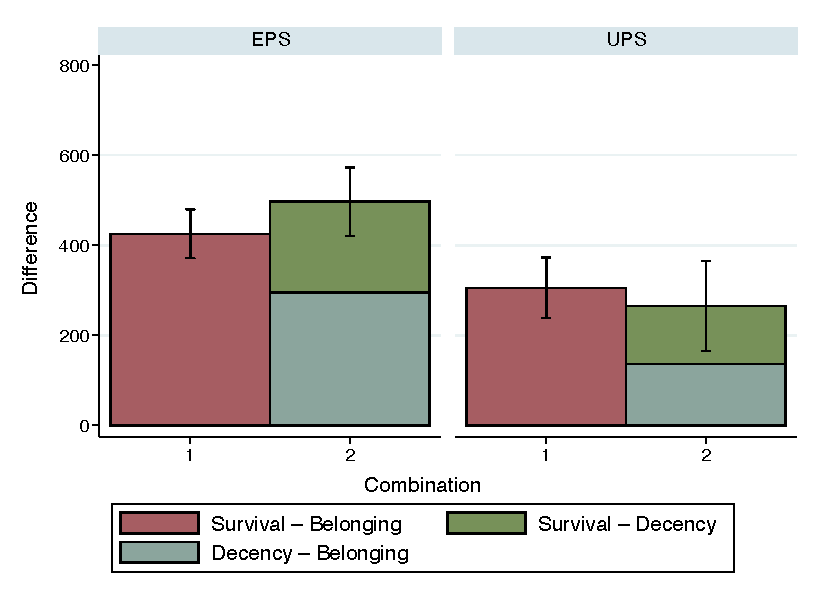
\includegraphics[width=.75\textwidth]{figures/figure_8.pdf}
   \begin{minipage}{0.75\linewidth}
   \footnotesize
   \emph{The figure shows a comparison between the reference case ``Survival -- Belonging'' and the possible addition by Productivity Scenario. $n = 200$.}
   \end{minipage}	
   \caption{Additivity of importance ratings: Survival -- Belonging}
   \label{fig:additivity_sub_2}
\end{figure}

To assess whether the references and the additions do not differ significantly from each other in their accumulated difference (i.\,e., the sum of the individual differences), we ran a number of one-way ANOVAs with Bonferroni correction; one for every Productivity Scenario regarding the combinations shown in Figure \ref{fig:additivity_all} (Equal Productivity Scenario: $F(3, 796) = 2.24$, $p = 0.083$; Unequal Productivity Scenario: $F(3, 796) = 2.82$, $p = 0.038$) as well as regarding the combinations shown in Figure \ref{fig:additivity_sub_1} (Equal Productivity Scenario: $F(1, 398) = 0.320$, $p = 0.571$; Unequal Productivity Scenario: $F(1, 398) = 8.010$, $p = 0.005$) and \ref{fig:additivity_sub_2} (Equal Productivity Scenario: $F(1, 398) = 3.240 $, $p = 0.073$; Unequal Productivity Scenario: $F(1, 398) = 0.610$, $p = 0.437$).
The ANOVAs indicate that the additions have total values that do not differ significantly from the reference values, except for the combination of \textit{Decency -- Belonging} and \textit{Belonging -- Autonomy} compared to the reference of \textit{Decency -- Autonomy} in the Unequal Productivity Scenario (with $p = 0.005$, see Figure \ref{fig:additivity_sub_1}).

Although most of the differences between the combinations of need comparisons are insignificant and, therefore, additivity cannot be rejected, a certain response pattern seems to emerge.
In the Equal Productivity Scenario, a slight superadditivity can be seen, which increases with the number of comparisons combined (see, in particular, the left panel of Figure \ref{fig:additivity_all}).Analogously, there is a slight tendency towards subadditivity in the Unequal Productivity Scenario, which also seems to increase when multiple comparisons are combined (see, in particular, the right panel of Figure \ref{fig:additivity_all}).
It could thus be that the participants, in the scenario where Persons A and B exhibit the same productivity but different needs, basically grant the needier person a kind of ``bonus'' that \textit{accumulates} when several comparisons are combined.
The Unequal Productivity Scenario creates a situation where (too much) distribution towards the needier person is itself perceived as unjust in terms of equity and, therefore, the needier person receives a ``malus'' that also accumulates when several comparisons are combined.
An obvious explanation for this decision pattern would be a gain-loss domain effect (for further occurrences of a gain-loss domain effect in the context of need-based justice, see \citealt{weis_needs_2017}).


\subsection{Regressions}\label{sec:results_regressions}
Finally, we turn to a number of Tobit panel regressions, reported in Table \ref{tab:regressions} using the participants ID as the panel variable and the case number as the time variable.
We chose to use Tobit models since our dependent variable---the difference between the logs distributed to Persons A and B---contains two left censored and 80 right censored observations.
Here, the largest difference ($\Delta_{Sur - Aut}$) serves as our reference category.
Model 1 shows that all other cases are highly significant, as is the overall model.
The constant is $465.076$, thus in the base case \textit{Survival -- Autonomy} Person A receives on average $465$ logs more than Person B.
There is a clear order of the cases, whereby the difference to the case \textit{Belonging -- Autonomy} is, as expected, the strongest with a regression coefficient amounting to $-416.201$.
Therefore, the average number of logs allotted to Person B is lower than the amount allotted to Person A in every case.

In Model 2, we added the Productivity variable and let it interact with the Case variable.
This shows that Productivity has a highly significant effect insofar as low productivity leads to a lower distribution to Person A (the difference between Person A and Person B decreases by $135$ logs).
This effect, as can be seen from the non-significant interaction terms, is not limited to individual cases, but rather related to the entire productivity block in each case.

Additionally, a pairwise comparison of margins was estimated for all combinations of differences that can be made with our four kinds of needs (see Table \ref{tab:pairwise} in Appendix \ref{sec:app_additional_tables}).
All but two comparisons are highly significant.

Model 3, then, shows that the two formulations---one of them in terms of avoidance of harm, the other one in terms of enablement of something good---make no overall difference. It has to be noted, though, that the interaction of Productivity Scenario and Formulation is weakly significant, amounting to a regression coefficient of $39.876$.

In Model 4, we add household net income, gender, and age, as well as political attitude and the importance of productivity, equality, and need, for the participants' decisions as control variables (these covariates are reported in Table \ref{tab:regression_cov} in Appendix \ref{sec:app_additional_tables}).
Of the covariates, only the questions for the importance of need, productivity, and equality as decision criteria are significant.
Here, stronger emphasis on the importance of productivity leads to a smaller difference between the logs distributed to Persons A and B with a regression coefficient of $-78.682$, so does---to a lesser extent---an emphasis on the importance of equality with a coefficient of $-16.959$.
Importance of need, then, works in the opposite direction, leading to a larger difference with a coefficient of $21.637$.

\begin{table}[ht!]
\centering
\caption{Allocation difference between Person A and B: Regression Results}
\label{tab:regressions}
\begin{tabular}{ld{3.6}d{3.6}d{3.6}d{3.6}}
   \hline\hline
                                       & \multicolumn{1}{c}{(1)}   & \multicolumn{1}{c}{(2)}   & \multicolumn{1}{c}{(3)}   & \multicolumn{1}{c}{(4)}   \\
   \hline
   Survival -- Belonging               &  -92.993^{***}      &  -99.337^{***}      &  -92.927^{***}      &  -98.491^{***}                              \\
                                       &  (19.569)           &  (26.790)           &  (18.920)           &  (20.198)                                   \\
   [1em]
   Decency – Autonomy                  & -134.304^{***}      & -127.306^{***}      & -134.295^{***}      & -138.839^{***}                              \\
                                       &  (19.563)           &  (26.776)           &  (18.914)           &  (20.190)                                   \\
   [1em]
   Decency – Belonging                 & -246.405^{***}      & -233.661^{***}      & -246.254^{***}      & -261.238^{***}                              \\
                                       &  (19.540)           &  (26.742)           &  (18.892)           &  (20.165)                                   \\
   [1em]
   Survival – Decency                  & -298.108^{***}      & -329.228^{***}      & -297.954^{***}      & -301.307^{***}                              \\
                                       &  (19.534)           &  (26.728)           &  (18.886)           &  (20.159)                                   \\
   [1em]
   Belonging – Autonomy                & -416.201^{***}      & -408.574^{***}      & -416.059^{***}      & -415.070^{***}                              \\
                                       &  (19.530)           &  (26.719)           &  (18.882)           &  (20.154)                                   \\
   [1em]
   Productivity                        &                     & -134.817^{***}      & -151.202^{***}      & -142.311^{***}                              \\
   $\{0=Equal, 1=Unequal\}$	           &                     &  (26.799)           &  (15.384)           &  (11.614)                                   \\
   [1em]
   Formulation                         &                     &                     &  -39.546            &  -25.407                                    \\
   $\{0=Avoidance, 1=Enablement\}$     &                     &                     &  (37.168)           &  (31.091)                                   \\
   [1em]
   Constant                            &  465.076^{***}      &  532.282^{***}      &  550.268^{***}      &  758.614^{***}                              \\
                                       &  (21.856)           &  (25.458)           &  (29.003)           & (155.900)                                   \\
   \hline
   Control variables                   & No                  &  No                 & No                  & Yes                                         \\
   Interaction between Productivity                                                                                                                    \\
   \hspace*{5mm}and Need Combination   & No                  &  Yes                & No                  & No                                          \\
   Interaction between Productivity                                                                                                                    \\
   \hspace*{5mm}and Formulation        & No                  &  No                 & Yes                 & No                                          \\
   \hline
   $\sigma_u$                          &  238.797^{***}      &  239.374^{***}      &  239.152^{***}      &  188.017^{***}                              \\
                                       &  (13.334)           &  (13.266)           &  (13.259)           &  (11.626)                                   \\
   $\sigma_e$                          &  274.654^{***}      &  265.281^{***}      &  265.513^{***}      &  270.947^{***}                              \\
                                       &   (4.238)           &   (4.094)           &   (4.097)           &   (4.377)                                   \\
   $\chi^2$                            &  600.020^{***}      &  794.280^{***}      &  789.480^{***}      &  817.420^{***}                              \\
   \hline
   \multicolumn{5}{p{\textwidth}}{\footnotesize \textit{The table reports the results of a Tobit random-effects panel regression. Endogenous variable: Allocation difference between A and B ($\Delta_A$). First row: coefficients, second row: standard errors in parentheses. Control variables include Age, Gender, and Household Net Income (see Table \ref{tab:regression_cov} in the Appendix). $N=2400$ ($200$ participants). 2 (80) left-censored (right-censored) observations. Significance levels: $^{*}$ $p < 0.10$, $^{**}$ $p < 0.05$, $^{***}$ $p < 0.01$.}}\\
   \end{tabular}
\end{table}


%%%%%%%%%%%%%%
% CONCLUSION %
%%%%%%%%%%%%%%
\section{Conclusion}\label{sec:conclusion}
In this paper, we presented the results of two vignette studies with online samples of the German adult population, investigating how laypeople evaluate four different kinds of needs, namely, survival, decency, belonging, and autonomy.
Participants of both studies were recruited via the online platform respondi.
Samples were stratified by gender, age, and income.

In the first study, participants ($n = 100$) had to evaluate the importance of the different kinds of needs in absolute terms on a 7-point Likert scale.
To this end, they were first presented with vignettes in which hypothetical persons experienced the different kinds of needs.
Each vignette was accompanied by an illustration.
We hypothesized that the four kinds of needs would not be perceived as equally important, but that there would be a hierarchy.
This hypothesis receives very clear support from the data; survival is rated highest, decency comes second, followed by belonging and autonomy.

In the second study, participants ($n = 200$) had to make distributive decisions.
They were presented with a series of cases in which two hypothetical persons experienced (mostly) different kinds of needs.
They then had to decide how to divide a scarce amount of a good between the two.
That is, they had to trade-off the satisfaction of one kind of need with another kind of need.
Within-participants, we have also varied whether the two persons contributed equally or differently to the amount available for (re)distribution.
Between-participants, we have further varied whether the kinds of needs were presented in an avoidance or enablement formulation.
The results lend further support to the hierarchy found in Study 1.
Additionally, we can see that the productivity of the two hypothetical persons has an influence on how participants distribute.
If one person has contributed less to the available amount, they tend to receive less of it.
In addition, we were able to verify that the distribution decisions of our participants are internally coherent insofar as they are additive.
Moreover, the type of formulation had no influence on the distribution of our participants, which shows that the effects found do not depend on minor differences in the wording.

Our results fit well with the hierarchizations from the psychological and philosophical literature. There are, of course, differences in the details, but the general orientation is quite similar.
When Alderfer proposes the triptych of existence needs, relatedness needs, and growth needs, or when Maslow suggests physiological needs, safety needs, social needs, esteem needs, and self-actualization needs, this comes fairly close to the ordering we found for our survival needs, decency needs, belonging needs, and autonomy needs.
Moreover, this ordering echoes the widespread idea from the philosophical literature that there are basic needs beyond the physiological minimum that must not be ignored just because survival comes first.
These needs are taken to be directed at social participation and human development.
Lastly, our results have interesting implications for the role of both needs and different justice principles in the context of distributive and social policy.
Our results show that, even in the case of the most basic needs, productivity still plays a role in distributive decisions, indicating that participants prefer social policies that are not unconditional but require a certain contribution.
Differentiating both with regard to the kinds of needs and to the contribution (and further factors of accountability, see \citealt{bauer_need_2022}) might be worthwhile in researching the relation of perceived deservingness and policy support (see, e.\,g., \citealt{gielens_deservingness_2019}, \citealt{heuer_unravelling_2020}).


%%%%%%%%%%%%%%%%
% BIBLIOGRAPHY %
%%%%%%%%%%%%%%%%
\clearpage
\bibliographystyle{elsarticle-harv}
\bibliography{references}


%%%%%%%%%%%%
% APPENDIX %
%%%%%%%%%%%%
\clearpage
\appendix


%%%%%%%%%%%%%%%%%%%%%%%%%%%
% INSTRUCTIONS OF STUDY 1 %
%%%%%%%%%%%%%%%%%%%%%%%%%%%
\section{Instructions of Study 1}\label{sec:app_study_1_instructions}
\subsection*{Welcome Screen}
In this survey, we are interested in your personal opinion and judgment. % In dieser Umfrage sind wir an Ihrer Meinung und Ihren Einschätzungen interessiert.
Therefore, there are no correct or incorrect answers in this study. % Es gibt in dieser Studie daher keine richtigen oder falschen Antworten.
Taking part in this study is voluntary, and you can drop out at any time. % Die Teilnahme an dieser Studie ist freiwillig, sie kann jederzeit abgebrochen werden.

You will probably need about 15 minutes if you work intently. % Bei konzentrierter Bearbeitung werden Sie voraussichtlich etwa 15 Minuten brauchen.
It is important that you complete the study without interruption and without closing your browser. % Es ist wichtig, dass Sie die Studie ohne Unterbrechung bearbeiten und ohne den Browser zwischendurch zu schließen.
If you cannot avoid closing your browser, you can continue the study by clicking on the link in the invitation at Mingle again. % Falls Sie ein Schließen des Browsers nicht vermeiden können, lässt sich die Studie fortsetzen, indem Sie erneut auf den Link bei Mingle klicken.

In the course of the study, we will give you a total of three attention checks. % Im Laufe der Studie werden wir Ihnen insgesamt drei Aufmerksamkeitsfragen stellen.
With these questions we want to make sure that you read and understand the instructions correctly. % Mit diesen Fragen möchten wir sicherstellen, dass Sie die Instruktionen korrekt lesen und verstehen.
If you answer more than one of these questions incorrectly, you will automatically be excluded from the study. % Wenn Sie mehr als eine dieser Fragen falsch beantworten, werden Sie automatisch aus der Studie ausgeschlossen.

We will analyze your answers together with the answers of all other participants in this study. % Wir werden Ihre Antworten sowie die Antworten aller anderen Teilnehmerinnen und Teilnehmer dieser Studie auswerten.
All data will be stored in an anonymous format so that no participant can be identified. % Alle Daten werden in anonymisierter Form gespeichert, so dass keine Angaben einer Person zugeordnet werden können.
The results of the study will be published. % Die Ergebnisse der Studie werden veröffentlicht.
They may influence future research and may be used to inform policymakers. % Diese beeinflussen damit zukünftige Forschung und sollen dazu genutzt werden, die Politik zu informieren.

Thank you for participation! % Vielen Dank für Ihre Teilnahme!


\subsection*{Vignette Text}
\noindent\textit{Note: We randomized the names displayed, denoted as $A$, $B$, $C$, and $D$ below (``Bauer'', ``Becker'', ``Fischer'', ``Hoffmann'', ``Klein'', ``Koch'', ``Meyer'', ``Müller'', ``Neumann'', ``Richter'', ``Schäfer'', ``Schmidt'', ``Schneider'', ``Schröder'', ``Schulz'', ``Schwarz'', ``Wagner'', ``Weber'', ``Wolf'', and ``Zimmermann'', based on frequent German surnames), as well as the order the four kinds of needs appeared in.
Next to each kind of need, a thumbnail of the picture illustrating this kind of need was displayed.}\vspace{2ex}

\noindent Please imagine four people with the names $A$, $B$, $C$, and $D$. % Bitte stellen Sie sich vier Personen mit den Namen $A$, $B$, $C$ und $D$ vor.
All are in need for wood. % Jede dieser Personen benötigt Feuerholz.
They need the wood for different reasons. % Sie benötigen das Feuerholz aus unterschiedlichen Gründen.
On this page, we present to you the different reasons for which $A$, $B$, $C$, and $D$ need the wood. % Auf dieser Seite stellen wir Ihnen vor, wofür $A$, $B$, $C$ und $D$ das Feuerholz jeweils benötigen.
On the following pages, you will be asked how important it is that the respective person's need is met.\vspace{2ex} % Auf den kommenden Seiten werden wir Sie fragen, für wie wichtig Sie es halten, dass der Bedarf dieser Personen erfüllt wird.

\noindent\textbf{A:} $A$ needs the wood to make sure to survive the coming winter. % $A$ benötigt das Holz, um sicherzustellen, dass er den kommenden Winter überlebt.
If $A$ receives less than he needs, it will be so cold in his hut that he is very likely to become life-threateningly ill. % Wenn $A$ weniger erhält als er braucht, wird es in seiner Hütte so kalt, dass er mit hoher Wahrscheinlichkeit lebensbedrohlich erkrankt.
The less wood he receives, the higher the probability that he will become life-threateningly ill.\vspace{2ex} % Je weniger Holz er erhält, desto höher ist die Wahrscheinlichkeit, dass er lebensbedrohlich erkrankt.

\noindent\textbf{B:} $B$ needs the wood in order not to freeze in the coming winter. % $B$ benötigt das Holz, um im kommenden Winter nicht zu frieren.
The members of the community to which $B$ belongs agree that one cannot live in dignity if one has to freeze. % Die Mitglieder der Gemeinde, zu der $B$ gehört, sind sich darin einig, dass man nicht in Würde leben kann, wenn man frieren muss.
If $B$ receives less than he needs, it becomes unacceptably cold in his hut. % Wenn $B$ weniger erhält als er braucht, wird es in seiner Hütte unannehmbar kalt.
The less wood he receives, the more often he will freeze.\vspace{2ex} % Je weniger Holz er erhält, desto häufiger wird er frieren.

\noindent\textbf{C:} $C$ needs the wood to be able to participate regularly in the social life of his community in the coming winter. % $C$ benötigt das Holz, um im kommenden Winter regelmäßig am sozialen Leben seiner Gemeinde teilhaben zu können.
It is common practice to meet at the community center and everyone brings wood with which to heat it. % Es ist Gang und Gäbe, dass man sich im Gemeindehaus trifft und jeder Holz mitbringt, mit dem es beheizt werden kann.
If $C$ receives less than he needs, he will not be able to participate regularly in the social life. % Wenn $C$ weniger erhält als er braucht, wird er nicht regelmäßig am sozialen Leben teilhaben können.
The less wood he receives, the less often he will be able to come to meetings at the community center.\vspace{2ex} % Je weniger Holz er erhält, desto seltener wird er zu Treffen im Gemeindehaus kommen können.

\noindent\textbf{D:} $D$ needs the wood to be able to use his studio regularly in the coming winter. % $D$ benötigt das Holz, um im kommenden Winter regelmäßig sein Atelier nutzen zu können.
He creates art there in his spare time. % Dort schafft er in seiner Freizeit Kunst.
If $D$ receives less than he needs, he will not be able to use his studio regularly. % Wenn $D$ weniger erhält als er braucht, wird er nicht regelmäßig sein Atelier nutzen können.
The less wood he receives, the less often he will be able to create art in his studio.\vspace{2ex} % Je weniger Holz er erhält, desto seltener wird er in seinem Atelier Kunst schaffen können.


\subsection*{Task}
\noindent\textit{Note: The needs of Person $A$, $B$, $C$, and $D$ were displayed on separate screens.
Their names were identical to those from the instructions screen.
The order of the four screens was randomized.
On each screen, we displayed a picture illustrating the kind of need in question.
Bellow each picture, a single sentence summed up the kind of need.
Participants had to enter their rating on a scale from 1 to 7.
An additional option for ``no answer/I don't know'' was included.}\vspace{2ex}

\noindent Please indicate how important you think the following kind of need is that $A$ ($B$, $C$, $D$) can meet by using firewood.\vspace{2ex} % Bitte geben Sie an, für wie wichtig Sie die folgende Art von Bedarf halten, die $A$ ($B$, $C$, $D$) mithilfe von Feuerholz decken kann.

\noindent\textbf{A:} $A$ needs the wood to avoid becoming life-threateningly ill.\vspace{2ex} % $A$ benötigt das Holz, um nicht lebensbedrohlich zu erkranken.

\noindent\textbf{B:} $B$ needs the wood to avoid freezing.\vspace{2ex} % $B$ benötigt das Holz, um nicht zu frieren.

\noindent\textbf{C:} $C$ needs the wood to participate in social life.\vspace{2ex} % $C$ benötigt das Holz, um am Sozialleben teilhaben zu können.

\noindent\textbf{D:} $D$ needs the wood to use his studio.\vspace{2ex} % $D$ benötigt das Holz, um sein Atelier nutzen zu können.

\noindent How much does $A$ $[B$, $C$, $D]$ need the wood in this case? % Wie sehr braucht $A$ ($B$, $C$, $D$) das Holz in diesem Fall?
Please give your answer on the following scale from 1 (``Does not need the wood at all'') to 7 (``Does absolutely need the wood''). % Bitte geben Sie Ihre Antwort auf der folgenden Skala von 1 (``Braucht das Holz überhaupt nicht'') bis 7 (``Braucht das Holz unbedingt'').


%%%%%%%%%%%%%%%%%%%%%%%%%%%%%%%%
% CONTROL QUESTIONS OF STUDY 1 %
%%%%%%%%%%%%%%%%%%%%%%%%%%%%%%%%
\clearpage
\section{Control Questions of Study 1}\label{sec:app_study_1_questions}
\noindent\textit{Note: Options for Questions 2 and 3 were displayed in randomized order.}\vspace{2ex}

\noindent\textbf{Question 1:} Please describe how often you reflect on justice issues in your daily life and what this means to you. % Bitte beschreiben Sie, wie oft Sie über Gerechtigkeitsfragen in Ihrem Alltag nachdenken und welche Bedeutung dies für Sie hat.

We ask this question to ensure that the tasks are read carefully. % Wir stellen diese Frage, um sichergehen zu können, dass die Aufgabenstellungen richtig gelesen werden.
If you are reading this, please enter the number 42 in the field below instead of an answer to the question itself. % Wenn Sie dies hier lesen, geben Sie bitte im untenstehenden Feld statt einer Antwort auf die eigentliche Fragestellung die Zahl 42 ein.

Have you ever reflected on justice issues?\vspace{1ex} % Haben Sie sich schon einmal mit Gerechtigkeitsfragen beschäftigt?

\noindent\textbf{Question 2:} How many reasons to need wood have we presented to you? % Wieviele verschiedene Gründe, Holz zu benötigen, haben wir Ihnen vorgestellt?
\begin{itemize}
   \item[$\square$] 3
   \item[$\square$] 4
   \item[$\square$] 5
\end{itemize}
\vspace{1ex}

\noindent\textbf{Question 3:} Which statements apply to this study? % Welche Aussagen treffen auf diese Studie zu?
Multiple answers are possible. % Mehrfachantworten sind möglich.
\begin{itemize}
   \item[$\square$] Wood is needed to renovate a building. % Holz wird benötigt, um ein Gebäude zu renovieren.
   \item[$\square$] Wood is needed to carve together. % Holz wird benötigt, um gemeinsam zu schnitzen.
   \item[$\square$] Wood is needed to heat. % Holz wird benötigt, um zu heizen.
\end{itemize}


%%%%%%%%%%%%%%%%%%%%%%%%%%%%%%%%%%%
% ADDITIONAL QUESTIONS OF STUDY 1 %
%%%%%%%%%%%%%%%%%%%%%%%%%%%%%%%%%%%
\clearpage
\section{Additional Questions of Study 1}\label{sec:app_study_1_additional_questions}
\subsection*{Political Orientation}
\noindent\textit{Note: An additional option for ``no answer/I don't know'' was included.}\vspace{1ex}

\noindent In politics, one speaks of left-wing and right-wing. % In der Politik spricht man von links und rechts.
How would you describe your own political position in general? % Wie würden Sie ganz allgemein Ihren eigenen politischen Standort beschreiben?
Where on a scale of 1 (left) to 7 (right) would you place yourself? % Wo auf einer Skala von 1 (links) bis 7 (rechts) würden Sie sich selbst einstufen?

\subsection*{Sensitivity to Cold}
\noindent\textit{Note: An additional option for ``no answer/I don't know'' was included.}\vspace{1ex}

\noindent On a scale from 1 (not at all sensitive to cold) to 7 (very sensitive to cold), how sensitive are you to cold? % Wie kälteempfindlich sind Sie auf einer Skala von "1 (überhaupt nicht kälteempfindlich) bis 7 (sehr kälteempfindlich)?


%%%%%%%%%%%%%%%%%%%%%%%%%%%
% INSTRUCTIONS OF STUDY 2 %
%%%%%%%%%%%%%%%%%%%%%%%%%%%
\clearpage
\section{Instructions of Study 2}\label{sec:app_study_2_instructions}
\subsection*{Welcome Screen}
In this survey, we are interested in your personal opinion and judgment. % In dieser Umfrage sind wir an Ihrer Meinung und Ihren Einschätzungen interessiert.
Therefore, there are no correct or incorrect answers in this study. % Es gibt in dieser Studie daher keine richtigen oder falschen Antworten.
Taking part in this study is voluntary, and you can drop out at any time. % Die Teilnahme an dieser Studie ist freiwillig, sie kann jederzeit abgebrochen werden.

You will probably need about 30 minutes if you work intently. % Bei konzentrierter Bearbeitung werden Sie voraussichtlich etwa 30 Minuten brauchen.
It is important that you complete the study without interruption and without closing your browser. % Es ist wichtig, dass Sie die Studie ohne Unterbrechung bearbeiten und ohne den Browser zwischendurch zu schließen.
If you cannot avoid closing your browser, you can continue the study by clicking on the link in the invitation at Mingle again. % Falls Sie ein Schließen des Browsers nicht vermeiden können, lässt sich die Studie fortsetzen, indem Sie erneut auf den Link bei Mingle klicken.

In the course of the study, we will give you a total of three attention checks. % Im Laufe der Studie werden wir Ihnen insgesamt drei Aufmerksamkeitsfragen stellen.
With these questions we want to make sure that you read and understand the instructions correctly. % Mit diesen Fragen möchten wir sicherstellen, dass Sie die Instruktionen korrekt lesen und verstehen.
If you answer more than one of these questions incorrectly, you will automatically be excluded from the study. % Wenn Sie mehr als eine dieser Fragen falsch beantworten, werden Sie automatisch aus der Studie ausgeschlossen.

We will analyze your answers together with the answers of all other participants in this study. % Wir werden Ihre Antworten sowie die Antworten aller anderen Teilnehmerinnen und Teilnehmer dieser Studie auswerten.
All data will be stored in an anonymous format so that no participant can be identified. % Alle Daten werden in anonymisierter Form gespeichert, so dass keine Angaben einer Person zugeordnet werden können.
The results of the study will be published. % Die Ergebnisse der Studie werden veröffentlicht.
They may influence future research and may be used to inform policymakers. % Diese beeinflussen damit zukünftige Forschung und sollen dazu genutzt werden, die Politik zu informieren.

Thank you for participation! % Vielen Dank für Ihre Teilnahme!

\subsection*{Instructions}
Your task will be to distribute firewood between two people. % Sie werden gleich gebeten, Feuerholz auf zwei Personen zu verteilen.
We will present you with a number of different scenarios and ask you to imagine that they are real. % Wir werden Ihnen dazu eine Reihe von unterschiedlichen Szenarien präsentieren und möchten Sie bitten, sich diese jeweils als real vorzustellen.
Please take the time to put yourself in the position of the scenarios and come to a personal judgment.  %Bitte nehmen Sie sich die Zeit, sich in die Szenarien hineinzuversetzen und zu einer persönlichen Einschätzung zu kommen.

\subsection*{Vignette Text}
\noindent\textit{Note: The four reasons were displayed to participants either in the Avoidance or in the Enablement Formulation.
We randomized the names displayed, denoted as $A$ and $B$ below (``Bauer'', ``Müller'', ``Schmidt'', ``Schneider'', ``Fischer'', ``Weber'', and ``Meyer'', based on frequent German surnames), as well as the position of the two persons (randomizing whether the more productive or the more needy person appears on the left side of the screen).}\vspace{2ex}

\noindent Please imagine two people with the names $A$ and $B$. % Bitte stellen Sie sich zwei Personen mit den Namen A und B vor.
$A$ and $B$ do not know each other. % A und B kennen sich nicht.
Both are in need of wood. % Beide benötigen Holz.
The community of $A$ and $B$ allows them to chop wood in the community forest for a certain period of time. % Die Gemeinde von A und B hat den beiden ermöglicht, in einem bestimmten Zeitraum im gemeindeeigenen Wald Holz zu schlagen.
Both have little money and therefore have no other way to get wood. % Beide verfügen über wenig Geld und haben daher keine andere Möglichkeit, sich Holz zu besorgen.

On the coming pages, we will present you with a total of 14 cases where $A$ and $B$ need the wood for different reasons. % Wir werden Ihnen auf den kommenden Seiten insgesamt 14 Fälle vorstellen, in denen A und B das Holz aus verschiedenen Gründen benötigen.
On each page, we will tell you what $A$ needs the wood for and what $B$ needs the wood for. % Auf jeder Seite werden wir Ihnen sagen, wofür A das Holz benötigt und wofür B das Holz benötigt.
You will then be asked to divide the wood as fairly as possible between $A$ and $B$. % Sie werden dann gebeten, das Holz möglichst gerecht zwischen A und B aufzuteilen.

Please note that you have to make the following trade-off: % Beachten Sie, dass Sie dabei folgende Abwägung treffen müssen:
The more wood you give to one person, the less you can give to the other. % Je mehr Holz Sie einer Person geben, desto weniger können Sie der anderen Person geben.
It is not possible to completely meet the needs of both people at the same time. % Es ist nicht möglich, die Bedarfe beider Personen gleichzeitig vollständig zu erfüllen.
In each of the 14 cases, the available amount of wood will only be enough to completely cover the needs of one of the two people; the other person would then go away empty-handed. % Die vorhandene Holzmenge würde in jedem der 14 Fälle nur reichen, um den Bedarf einer der beiden Person gerade vollständig zu decken; die andere Person würde dann leer ausgehen.

We now present to you the four different reasons for which A and B may need the wood. % Wir stellen Ihnen nun die vier verschiedenen Gründe vor, aus denen A und B das Holz benötigen können.
These four reasons have to do with the coming winter. % Diese vier Gründe haben mit dem kommenden Winter zu tun.
Since you need to distribute the wood in advance without knowing exactly how cold the winter will be, we describe the expected effects of the winter on the people as more or less likely. % Da Sie das Holz im Voraus verteilen müssen, ohne zu wissen, wie kalt der Winter genau wird, geben wir die voraussichtlichen Auswirkungen des Winters auf die Personen als mehr oder weniger wahrscheinlich an.

Please read the descriptions of the four reasons carefully.\vspace{2ex} % Lesen Sie sich die Beschreibungen der vier Gründe bitte aufmerksam durch.

\noindent\textbf{Reason 1 (Avoidance Formulation):} The person needs the wood to avoid falling life-threateningly ill and dying from it in winter. % Die Person benötigt das Holz, um im Winter nicht lebensbedrohlich zu erkranken und daran zu sterben.
They heat their hut exclusively with wood. % Sie heizt ihre Hütte ausschließlich mit Holz.
The more logs the person gets, the less likely they are to fall life-threateningly ill. % Je mehr Holzscheite die Person bekommt, desto geringer ist die Wahrscheinlichkeit, dass sie lebensbedrohlich erkranken wird.
If the person gets no wood at all, they will certainly fall life-threateningly ill. % Wenn die Person gar kein Holz bekommt, wird sie mit Sicherheit lebensbedrohlich erkranken.
If the person gets all the available wood, they will certainly not fall life-threateningly ill.\vspace{2ex} % Wenn die Person alles verfügbare Holz bekommt, wird sie mit Sicherheit nicht lebensbedrohlich erkranken.

\noindent\textbf{Reason 1 (Enablement Formulation):} The person needs the wood to stay healthy and survive in winter. % Die Person benötigt das Holz, um im Winter gesund zu bleiben und zu überleben.
She heats her hut exclusively with wood. % Sie heizt ihre Hütte ausschließlich mit Holz.
The more logs the person gets, the higher the probability that they will stay healthy. % Je mehr Holzscheite die Person bekommt, desto höher ist die Wahrscheinlichkeit, dass sie gesund bleiben wird.
If the person gets no wood at all, they will certainly not stay healthy. % Wenn die Person gar kein Holz bekommt, wird sie mit Sicherheit nicht gesund bleiben.
If the person gets all the available wood, they will certainly stay healthy.\vspace{2ex} % Wenn die Person alles verfügbare Holz bekommt, wird sie mit Sicherheit gesund bleiben.

\noindent\textbf{Reason 2 (Avoidance Formulation):} The person needs the wood to not freeze in winter. % Die Person benötigt das Holz, um im Winter nicht zu frieren.
They heat their hut exclusively with wood. % Sie heizt ihre Hütte ausschließlich mit Holz.
The more logs the person gets, the less likely they will freeze. % Je mehr Holzscheite die Person bekommt, desto geringer ist die Wahrscheinlichkeit, dass sie frieren wird.
If the person gets no wood at all, they will certainly freeze. % Wenn die Person gar kein Holz bekommt, wird sie mit Sicherheit frieren.
If the person gets all the wood available, they will certainly not freeze.\vspace{2ex} % Wenn die Person alles verfügbare Holz bekommt, wird sie mit Sicherheit nicht frieren.

\noindent\textbf{Reason 2 (Enablement Formulation):} The person needs the wood to be warm in winter. % Die Person benötigt das Holz, um es im Winter warm zu haben.
They heat their hut exclusively with wood. % Sie heizt ihre Hütte ausschließlich mit Holz.
The more logs the person gets, the higher the probability that they will be warm. % Je mehr Holzscheite die Person bekommt, desto höher ist die Wahrscheinlichkeit, dass sie es warm haben wird.
If the person does not get any wood at all, they will certainly not have it warm. % Wenn die Person gar kein Holz bekommt, wird sie es mit Sicherheit nicht warm haben.
If the person gets all the available wood, they will certainly have it warm.\vspace{2ex} % Wenn die Person alles verfügbare Holz bekommt, wird sie es mit Sicherheit warm haben.

\noindent\textbf{Reason 3 (Avoidance Formulation):} The person needs the wood in order not to be excluded from social life in winter, since it is common practice to meet in the community center and everyone brings wood with which to heat it. % Person benötigt das Holz, um im Winter nicht vom sozialen Leben ausgeschlossen zu sein, da es Gang und Gäbe ist, dass man sich im Gemeindehaus trifft und jeder Holz mitbringt, mit dem das Gemeindehaus beheizt werden kann.
The more logs the person gets, the less likely they are to be excluded from social life. % Je mehr Holzscheite die Person bekommt, desto geringer ist die Wahrscheinlichkeit, dass sie vom sozialen Leben ausgeschlossen sein wird.
If the person gets no wood at all, they will certainly be excluded from social life. % Wenn die Person gar kein Holz bekommt, wird sie mit Sicherheit vom sozialen Leben ausgeschlossen sein.
If the person gets all the available wood, they will certainly not be excluded from social life.\vspace{2ex} % Wenn die Person alles verfügbare Holz bekommt, wird sie mit Sicherheit nicht vom sozialen Leben ausgeschlossen sein.

\noindent\textbf{Reason 3 (Enablement Formulation):} The person needs the wood to participate in social life in winter, since it is common practice to meet in the community center and everyone brings wood to heat it. % Die Person benötigt das Holz, um im Winter am sozialen Leben teilzuhaben, da es Gang und Gäbe ist, dass man sich im Gemeindehaus trifft und jeder Holz mitbringt, mit dem das Gemeindehaus beheizt werden kann.
The more logs the person gets, the more likely they are to participate in social life. % Je mehr Holzscheite die Person bekommt, desto höher ist die Wahrscheinlichkeit, dass sie am sozialen Leben teilhaben wird.
If the person does not get any wood at all, they will certainly not participate in social life. % Wenn die Person gar kein Holz bekommt, wird sie mit Sicherheit nicht am sozialen Leben teilhaben.
If the person gets all the available wood, they will certainly participate in social life.\vspace{2ex} % Wenn die Person alles verfügbare Holz bekommt, wird sie mit Sicherheit am sozialen Leben teilhaben.

\noindent\textbf{Reason 4 (Avoidance Formulation):} The person needs the wood so that their studio does not become unusable in winter. % Die Person benötigt das Holz, damit ihr Atelier im Winter nicht unbenutzbar wird.
They heat their studio exclusively with wood. % Sie heizt ihr Atelier ausschließlich mit Holz.
There, they create art in their free time. % Dort schafft sie in ihrer Freizeit Kunst.
The more logs the person gets, the less likely it is that their studio will become unusable. % Je mehr Holzscheite die Person bekommt, desto geringer ist die Wahrscheinlichkeit, dass ihr Atelier unbenutzbar wird.
If the person gets no wood at all, their studio will certainly be unusable. % Wenn die Person gar kein Holz bekommt, wird ihr Atelier mit Sicherheit unbenutzbar sein.
If the person gets all the available wood, their studio will certainly not be unusable.\vspace{2ex} % Wenn die Person alles verfügbare Holz bekommt, wird ihr Atelier mit Sicherheit nicht unbenutzbar sein.

\noindent\textbf{Reason 4 (Enablement Formulation):} The person needs the wood so that they can use their studio in the winter. % Die Person benötigt das Holz, damit sie ihr Atelier im Winter nutzen kann.
They heat their studio exclusively with wood. % Sie heizt ihr Atelier ausschließlich mit Holz.
There, they create art in their free time. % Dort schafft sie in ihrer Freizeit Kunst.
The more logs the person gets, the more likely they are to use their studio. % Je mehr Holzscheite die Person bekommt, desto höher ist die Wahrscheinlichkeit, dass sie ihr Atelier nutzen wird.
If the person gets no wood at all, they will certainly not use their studio. % Wenn die Person gar kein Holz bekommt, wird sie mit Sicherheit nicht ihr Atelier nutzen.
If the person gets all the available wood, they will certainly use their studio. % Wenn die Person alles verfügbare Holz bekommt, wird mit Sicherheit ihr Atelier nutzen.


\subsection*{Scenario Introduction}
\noindent\textit{Note: Before each scenario, a single sentence was displayed to introduce participants to the productivity of Person $A$ and $B$ in the next seven cases.}\vspace{2ex}

\noindent\textbf{Equal Productivity Scenario:} In the following 7 cases that we show you, $A$ and $B$ have each cut 500 logs of wood.\vspace{2ex} % In den folgenden 7 Fällen, die wir Ihnen zeigen, haben A und B haben jeweils 500 Holzscheite geschlagen.

\noindent\textbf{Unequal Productivity Scenario:} In the following 7 cases that we show you, A has cut 200 and B 800 logs of wood. % In den folgenden 7 Fällen, die wir Ihnen zeigen, hat A 200 und B 800 Holzscheite geschlagen.


\clearpage
\subsection*{Exemplary Task}
$A$ and $B$ have cut 500 logs each $[A$ has cut 200 and $B$ has cut 800 logs$]$. % A und B haben jeweils 500 Holzscheite geschlagen.
So both persons have cut a total of 1,000 logs. % Beide Personen haben also zusammengerechnet 1.000 Holzscheite geschlagen.
In the empty spaces below, please make the distribution to both people that you think is most just.\vspace{4ex} % Bitte nehmen Sie in den freien Feldern unten diejenige Verteilung auf beide Personen vor, die aus Ihrer Sicht am gerechtesten ist.

\begin{minipage}[t]{.4\linewidth}
   
\includegraphics[width=\linewidth]{figures/figure_1_d.jpg}
   $A$ needs the wood so that their studio does not become unusable in the winter.\\[2ex] $A$ should receive \_\_\_ logs of wood.
\end{minipage}
\hfill
\begin{minipage}[t]{.4\linewidth}
   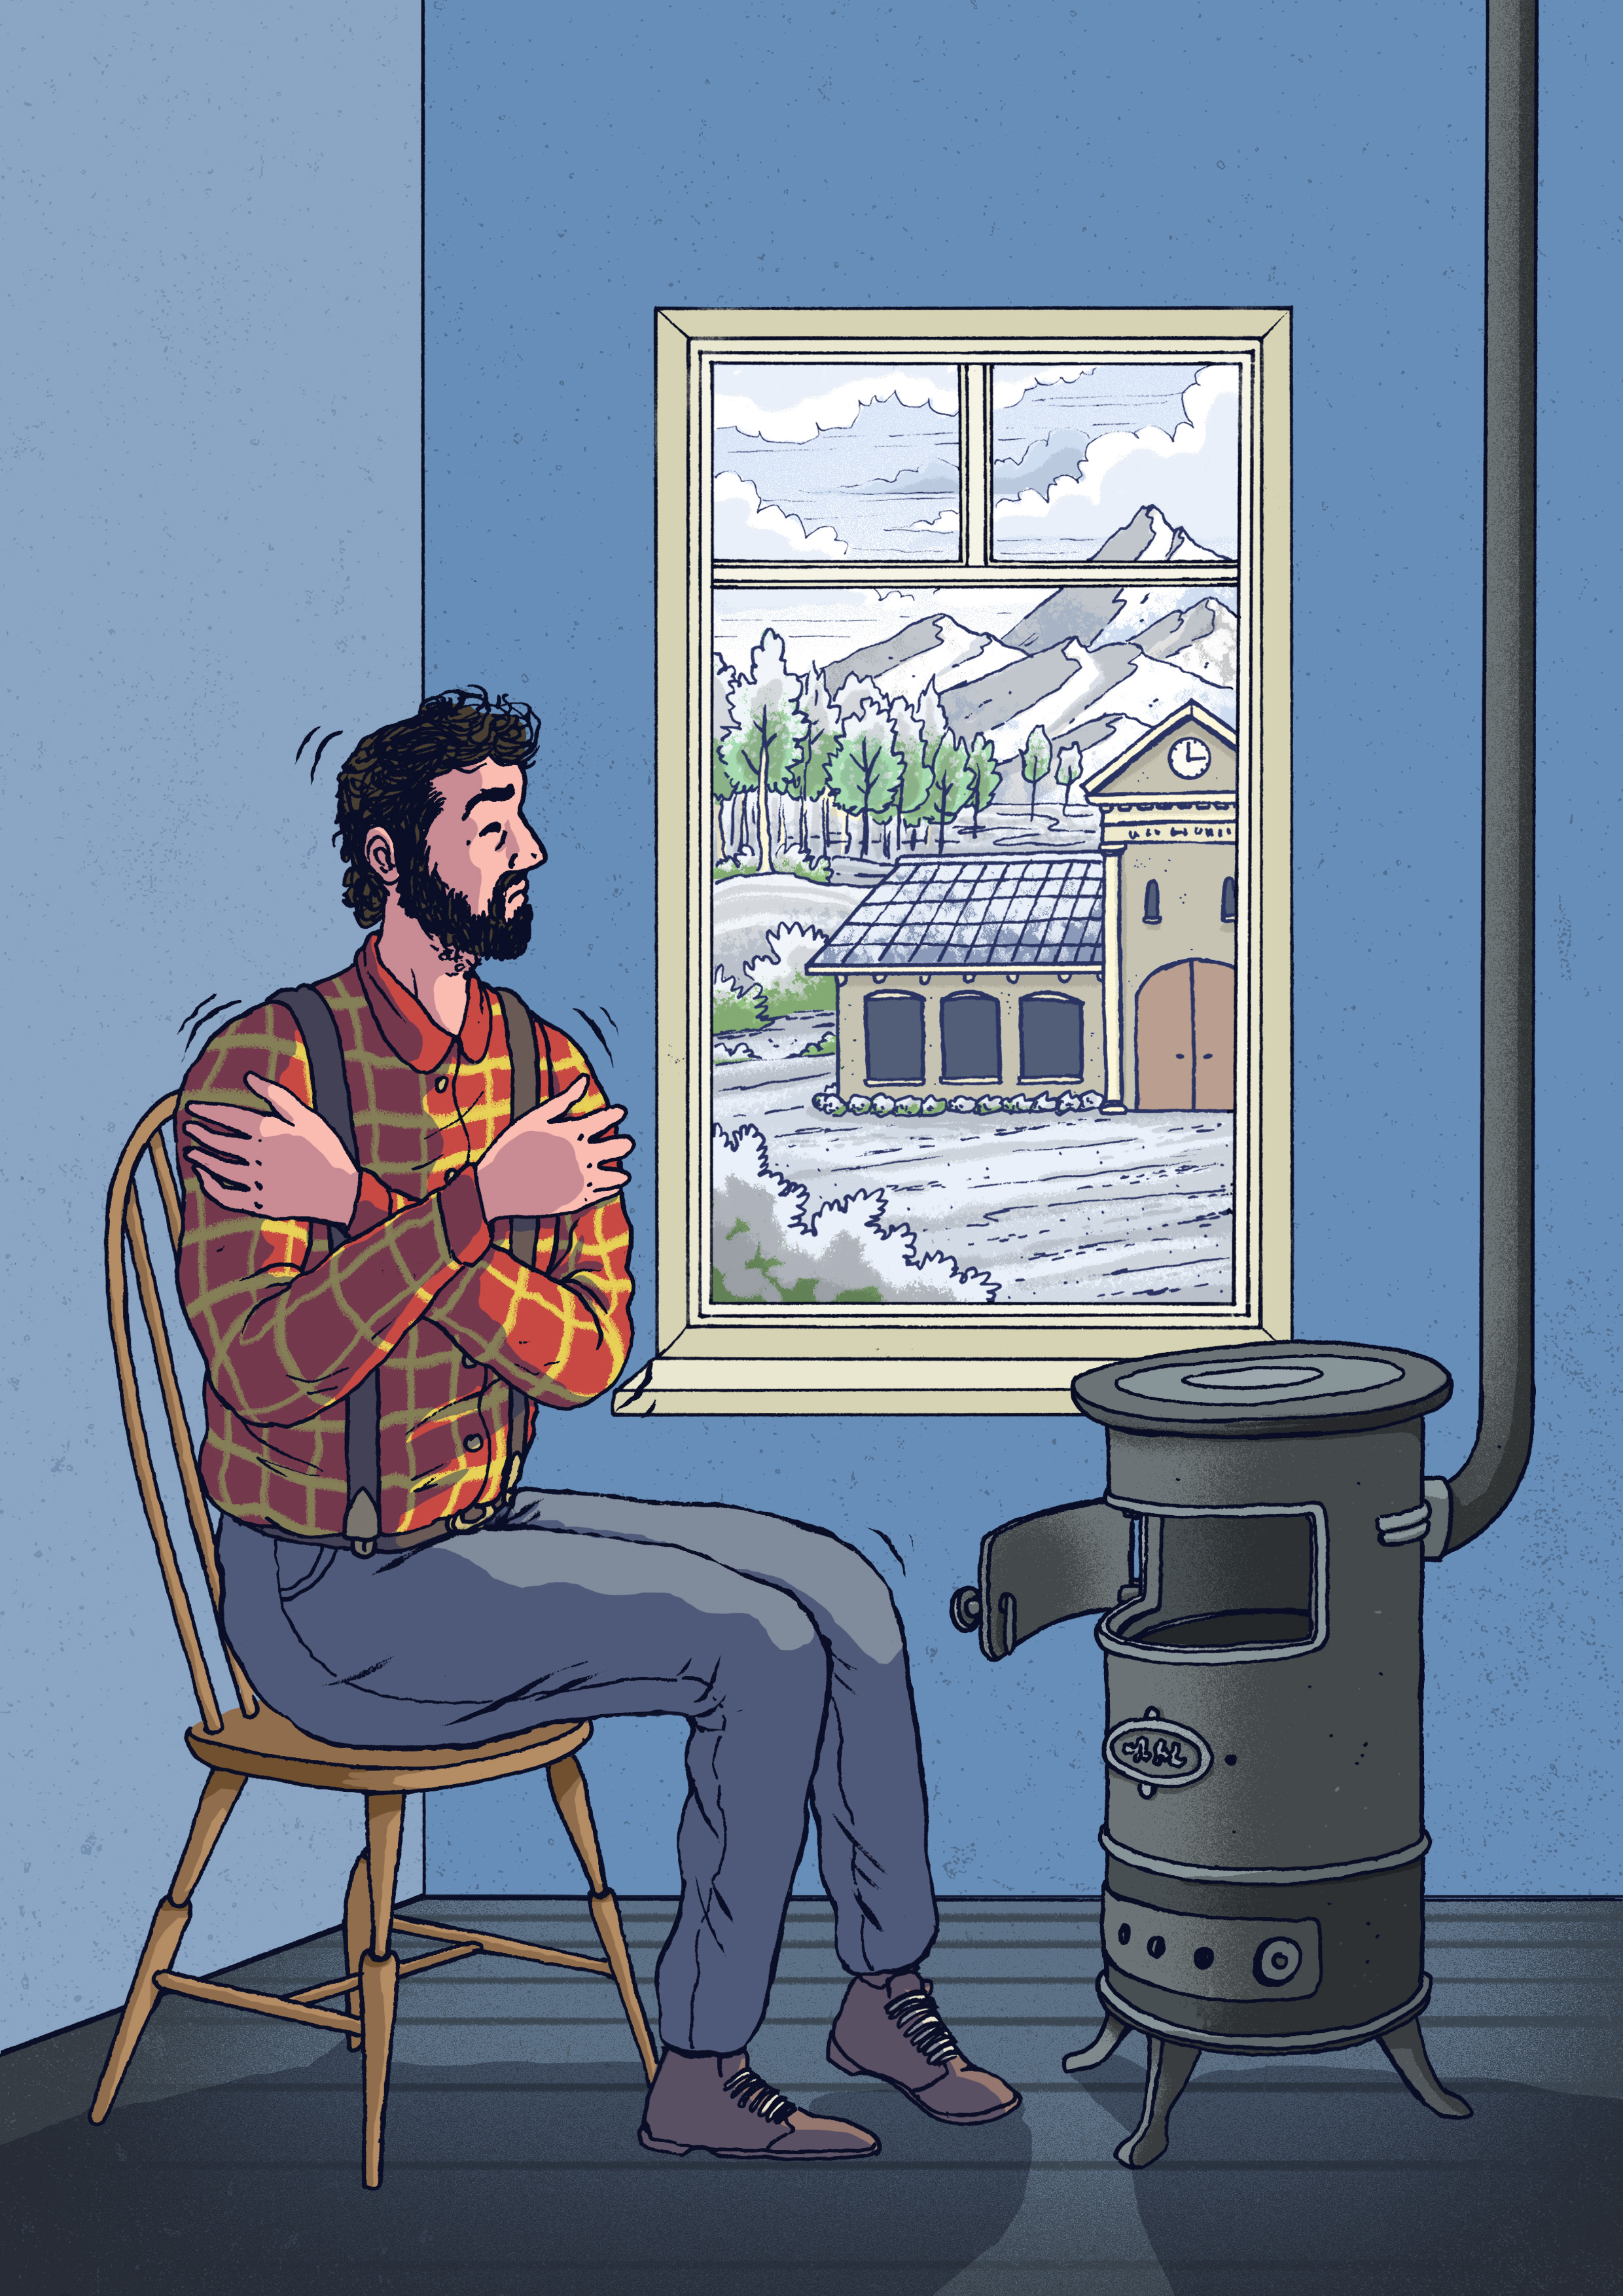
\includegraphics[width=\linewidth]{figures/figure_1_b.jpg}
   $B$ needs the wood to avoid freezing in the winter.\\[5ex] $B$ should receive \_\_\_ logs of wood.
\end{minipage}


%%%%%%%%%%%%%%%%%%%%%%%%%%%%%%%%
% CONTROL QUESTIONS OF STUDY 2 %
%%%%%%%%%%%%%%%%%%%%%%%%%%%%%%%%
\clearpage
\section{Control Questions of Study 2}\label{sec:app_study_2_control_questions}
\noindent\textit{Note: Options for Questions 2 and 3 were displayed in randomized order.}\vspace{1ex}

\noindent\textbf{Question 1:} Please describe how often you reflect on justice issues in your daily life and what this means to you. % Bitte beschreiben Sie, wie oft Sie über Gerechtigkeitsfragen in Ihrem Alltag nachdenken und welche Bedeutung dies für Sie hat.

We ask this question to ensure that the tasks are read carefully. % Wir stellen diese Frage, um sichergehen zu können, dass die Aufgabenstellungen richtig gelesen werden.
If you are reading this, please enter the number 42 in the field below instead of an answer to the question itself. % Wenn Sie dies hier lesen, geben Sie bitte im untenstehenden Feld statt einer Antwort auf die eigentliche Fragestellung die Zahl 42 ein.

Have you ever reflected on justice issues?\vspace{1ex} % Haben Sie sich schon einmal mit Gerechtigkeitsfragen beschäftigt?

\noindent\textbf{Question 2:} Which statements apply to this study? % Welche Aussagen treffen auf diese Studie zu?
Multiple answers are possible. % Mehrfachantworten sind möglich.

\begin{itemize}
   \item[$\square$] Farmers work a rye field. % Bauern bearbeiten ein Roggenfeld.
   \item[$\square$] Farmers work a sunflower field. % Bauern bearbeiten ein Sonnenblumenfeld.
   \item[$\square$] Farmers work a wheat field. % Bauern bearbeiten ein Weizenfeld.
   \item[$\square$] Wood is needed to build a house. % Holz wird benötigt, um ein Haus zu bauen.
   \item[$\square$] Wood is needed to heat in winter. % Holz wird benötigt, um im Winter zu heizen.
   \item[$\square$] Water is needed to run a mill. % Wasser wird benötigt, um eine Mühle anzutreiben.
   \item[$\square$] Water is needed to drink. % Wasser wird benötigt, um zu trinken.
\end{itemize}
\vspace{1ex}

\noindent\textbf{Question 3:} How much wood have $A$ and $B$ cut together in the previous displayed cases. % Wie viel Holz brauchten Schneider und Weber in den vorgestellten Fällen jeweils für sich genommen?

\begin{itemize}
   \item[$\square$] 5000
   \item[$\square$] 3000
   \item[$\square$] 2500
   \item[$\square$] 1800
   \item[$\square$] 1200
   \item[$\square$] 1000
   \item[$\square$] 500
\end{itemize}


%%%%%%%%%%%%%%%%%%%%%%%%%%%%%%%%%%%
% ADDITIONAL QUESTIONS OF STUDY 2 %
%%%%%%%%%%%%%%%%%%%%%%%%%%%%%%%%%%%
\clearpage
\section{Additional Questions of Study 2}\label{sec:app_study_2_additional_questions}
\subsection*{Support for Different Distribution Principles}
\noindent\textit{Note: Items were displayed in a randomized order. An additional option for ``no answer/I don't know'' was included.}\vspace{1ex}

\noindent How important were the following considerations for your distributions? % Wie wichtig waren die folgenden Überlegungen für Ihre Verteilungen?
Please give your answers on a scale from 1 (not at all important) to 7 (very important). % Bitte geben Sie Ihre Antworten auf einer Skala von 1 (überhaupt nicht wichtig) bis 7 (sehr wichtig).

\begin{itemize}
   \item Each person should receive as much wood as they need. % Jede Person sollte so viel Holz bekommen, wie sie braucht.
   \item Each person should receive the wood they have chopped. % Jede Person sollte das Holz bekommen, das sie geschlagen hat.
   \item Each person should receive the same amount of wood. % Jede Person sollte gleich viel Holz bekommen.
\end{itemize}

\subsection*{Political Orientation}
\noindent\textit{Note: An additional option for ``no answer/I don't know'' was included.}\vspace{1ex}

\noindent In politics, one speaks of left-wing and right-wing. % In der Politik spricht man von links und rechts.
How would you describe your own political position in general? % Wie würden Sie ganz allgemein Ihren eigenen politischen Standort beschreiben?
Where on a scale of 1 (left) to 7 (right) would you place yourself? % Wo auf einer Skala von 1 (links) bis 7 (rechts) würden Sie sich selbst einstufen?

\subsection*{Sensitivity to Cold}
\noindent\textit{Note: An additional option for ``no answer/I don't know'' was included.}\vspace{1ex}

\noindent On a scale from 1 (not at all sensitive to cold) to 7 (very sensitive to cold), how sensitive are you to cold? % Wie kälteempfindlich sind Sie auf einer Skala von "1 (überhaupt nicht kälteempfindlich) bis 7 (sehr kälteempfindlich)?


%%%%%%%%%%%%%%%%%%%%%
% ADDITIONAL TABLES %
%%%%%%%%%%%%%%%%%%%%%
\clearpage
\section{Additional Tables}\label{sec:app_additional_tables}

\begin{table}[ht!]
\center
\caption{Sample of Study 1 by Gender, Age, and Income}
\label{tab:quota_study_1}
\begin{tabular}{lrrrrr}\\[0.5ex]
   \hline
   \multicolumn{2}{c}{Gender}   & \multicolumn{2}{c}{Age}   & \multicolumn{2}{c}{Income Interval$^a$}   \\
   \hline
   Group    & Share             & Group	    & Share         & Group              & Share                \\
   \hline\hline
   Female   & 50.0              & $18-29$   & 21.0          &    [0, 1100)       & 16.0                 \\
   Male     & 50.0              & $30-39$   & 18.0          & [1100, 1500)       & 23.0                 \\
   	        &                   & $40-49$   & 19.0          & [1500, 2000)       & 23.0                 \\
   	        &                   & $50-59$   & 24.0          & [2000, 2600)       & 19.0                 \\
   	        &                   & $60-69$   & 18.0          & [2600, $\infty$)   & 19.0                 \\
   \hline
   \multicolumn{6}{p{9cm}}{\footnotesize{\textit{Share in percent. $n=100$. $^a$Equivalent household net income.}}}
\end{tabular}
\end{table}

\begin{landscape}
\begin{table}[ht!]
\center
\caption{Control variables for Study 1}
\label{tab:reg_study_1}
\begin{tabular}{ld{2.6}d{2.6}d{2.6}d{2.6}d{2.6}d{2.6}}\\[0.5ex]
   \hline
                               & \multicolumn{1}{c}{(1)}   & \multicolumn{1}{c}{(2)}   & \multicolumn{1}{c}{(3)}   & \multicolumn{1}{c}{(4)}   & \multicolumn{1}{c}{(5)}   & \multicolumn{1}{c}{(6)}   \\
   \hline\hline
   Decency                     &  -0.840^{***}             & -0.838^{***}              &  -2.706^{***}             &  -2.702^{***}             &  -0.834^{***}             &  -0.832^{***}             \\
                               &  (0.178)                  & (0.179)                   &  (0.319)                  &  (0.319)                  &  (0.105)                  &  (0.106)                  \\
   Belonging                   &  -2.779^{***}             & -2.780^{***}              &  -5.028^{***}             &  -5.024^{***}             &  -2.781^{***}             &  -2.782^{***}             \\
                               &  (0.178)                  & (0.179)                   &  (0.323)                  &  (0.322)                  &  (0.160)                  &  (0.161)                  \\
   Autonomy                    &  -3.530^{***}             & -3.530^{***}              &  -5.851^{***}             &  -5.847^{***}             &  -3.530^{***}             &  -3.530^{***}             \\
                               &  (0.178)                  & (0.178)                   &  (0.325)                  &  (0.324)                  &  (0.175)                  &  (0.176)                  \\
   Age                         &                           & -0.006                    &                           &  -0.008                   &                           &  -0.006                   \\
   $\{\sharp years\}$          &                           & (0.004)                   &                           &  (0.009)                  &                           &  (0.006)                  \\
   Gender                      &                           & -0.025                    &                           &   0.009                   &                           &  -0.021                   \\
   $\{0 = female,1 = male\}$   &                           & (0.136)                   &                           &  (0.281)                  &                           &  (0.181)                  \\
   Household Net Income        &                           & -1.14e^{-6}               &                           &  -1.36e^{-6}              &                           &  -1.14e^{-6}              \\
   $\{euros\}$                 &                           & (3.10e^{-6})              &                           &  (6.34e^{-6})             &                           &  (1.22e^{-6})             \\
   Political Attitude          &                           & -0.004                    &                           &  -0.006                   &                           &  -0.004^{***}             \\
   $\{1,\ldots,7\}$            &                           & (0.003)                   &                           &  (0.006)                  &                           &  (0.002)                  \\
   Sensitivity to Cold         &                           &  0.025                    &                           &   0.021                   &                           &   0.026                   \\
   $\{1,\ldots,7\}$            &                           & (0.046)                   &                           &  (0.095)                  &                           &  (0.062)                  \\
   Constant                    &   6.830^{***}             &  7.023^{***}              &   9.082^{***}             &   9.378^{***}             &   6.830^{***}             &   7.025^{***}             \\
                               &  (0.126)                  & (0.344)                   &  (0.305)                  &  (0.733)                  &  (0.065)                  &   0.472                   \\
   \hline
   $F$                         & 170.680^{***}             & 64.310^{***}              &                           &                           &                           &                           \\
   $\chi^2$                    &                           &                           & 440.56^{***}              & 441.890^{***}             & 453.470^{***}             & 709.130^{***}             \\
   \hline
   \multicolumn{7}{p{17cm}}{\footnotesize\textit{The table reports the results of two pooled OLS regressions (Models (1) and (2)), two Tobit panel regressions (Models (3) and (4)), as well as two random-effects GLS panel regressions (Models (5) and (6); panel variable: id). Endogenous variable: importance rating. First row: coefficients, second row: standard errors in parentheses. $n = 100$. Significance levels: $^{*}$ $p < 0.10$, $^{**}$ $p < 0.05$, $^{***}$ $p < 0.01$.}}
   \end{tabular}
\end{table}
\end{landscape}

\begin{table}[ht!]
\center
\caption{Contrasts of predictive margins for Study 1}
\label{tab:con_study_1}
\begin{tabular}{ld{1.3}d{1.3}d{2.6}}\\[0.5ex]
   \hline\hline
                   & \multicolumn{1}{c}{Contrast}   & \multicolumn{1}{c}{Std. Err.}   & \multicolumn{1}{c}{$t$}   \\
   Dec. vs. Sur.   & -0.838                         & 0.179                           &  -4.690^{***}             \\
   Bel. vs. Sur.   & -2.780                         & 0.179                           & -15.570^{***}             \\
   Aut. vs. Sur.   & -3.530                         & 0.178                           & -19.820^{***}             \\
   Bel. vs. Dec.   & -1.942                         & 0.179                           & -10.850^{***}             \\
   Aut. vs. Dec.   & -2.692                         & 0.179                           & -15.080^{***}             \\
   Aut. vs. Bel.   & -0.750                         & 0.179                           &  -4.200^{***}             \\
   \hline
   \multicolumn{4}{p{8.5cm}}{\footnotesize\textit{The table reports the contrasts of the predictive margins of the mean ratings of the four kinds of needs. $n = 100$. Significance levels: $^{*}$ $p < 0.10$, $^{**}$ $p < 0.05$, $^{***}$ $p < 0.01$.}}
   \end{tabular}
\end{table}

\begin{table}[ht!]
\center
\caption{Sample of Study 2 by Gender, Age, and Income}
\label{tab:quota_study_2}
\begin{tabular}{rrrrrr}\\[0.5ex]
   \hline
   \multicolumn{2}{c}{Gender}   & \multicolumn{2}{c}{Age}   & \multicolumn{2}{c}{Income Interval$^a$}   \\
   \hline
   Group    & Share             & Group     & Share         & Group              & Share                \\
   \hline\hline
   Female   & 50.0              & $18-29$   & 21.0          &    [0, 1100)       & 16.0                 \\
   Male	    & 50.0              & $30-39$   & 18.0          & [1100, 1500)       & 23.0                 \\
            &                   & $40-49$   & 19.0          & [1500, 2000)       & 23.0                 \\
            &                   & $50-59$   & 24.0          & [2000, 2600)       & 19.0                 \\
            &                   & $60-69$   & 18.0          & [2600, $\infty$)   & 19.0                 \\
   \hline
   \multicolumn{6}{p{8cm}}{\footnotesize\textit{Share in percent. $n=200$. $^a$Household net income.}}
\end{tabular}
\end{table}

\begin{table}[ht!]
\center
\caption{Percentage deviation of the share that Person A receives from the share that Person A contributed for Paired Cases by Productivity Scenario.}
\label{tab:means_deviation_paired}
\begin{tabular}{lcd{1.3}d{1.3}cd{1.3}d{1.3}}\\[0.5ex]
   \hline
                  &   & \multicolumn{5}{c}{Productivity Scenario}                                                                                             \\\cline{3-7}
                  &   & \multicolumn{2}{c}{EPS}   &   & \multicolumn{2}{c}{UPS}                                                                               \\\cline{3-4}\cline{6-7}
   Case           &   & \multicolumn{1}{c}{Mean \%}   & \multicolumn{1}{c}{Std. Dev.}   &   & \multicolumn{1}{c}{Mean \%}   & \multicolumn{1}{c}{Std. Dev.}   \\
   \hline\hline
   Sur. -- Sur.   &   &  0.741                        & 4.279                           &   & 10.556                        & 4.538                           \\
   Dec. -- Dec.   &   &  0.000                        & 0.000                           &   &  9.000                        & 4.678                           \\
   Bel. -- Bel.   &   &  0.698                        & 3.196                           &   &  6.791                        & 5.276                           \\
   Aut. -- Aut.   &   &  1.765                        & 8.867                           &   &  7.489                        & 6.037                           \\
   \hline
   \multicolumn{7}{p{10.5cm}}{\footnotesize\textit{The table reports means of absolute percentage deviations of the share that Person A receives from the share that Person A contributed for Paired Cases by Productivity Scenario.}}
\end{tabular}
\end{table}

\begin{landscape}
\begin{table}[ht!]
\center
\caption{Mean differences for Cases by Productivity Scenario.}
\label{tab:means_mixed_paired}
\begin{tabular}{lcd{3.3}ccd{3.3}cd{3.3}d{1.6}}\\[0.5ex]
   \hline
                  &   & \multicolumn{5}{c}{Productivity Scenario}                                                                                               &                             &                           \\\cline{3-7}
                  &   & \multicolumn{2}{c}{EPS}                                          &   & \multicolumn{2}{c}{UPS}                                          &                             &                           \\\cline{3-4}\cline{6-7}
   Case           &   & \multicolumn{1}{c}{$\Delta$}   & \multicolumn{1}{c}{$95\%$ CI}   &   & \multicolumn{1}{c}{$\Delta$}   & \multicolumn{1}{c}{$95\%$ CI}   & \multicolumn{1}{c}{Diff.}   & \multicolumn{1}{c}{$t$}   \\
   \hline\hline
   Sur. -- Sur.   &   & -14.8                          & $[-37.709,  8.080]$             &   &  -72.2                         & $[-132.921,  -11.523]$          &  57.4                       & 1.740^{*}                 \\
   Dec. -- Dec.   &   &   0.0                          &                                 &   & -150.0                         & $[-213.765,  -86.235]$          & 150.0                       & 4.625^{***}               \\
   Bel. -- Bel.   &   &   9.3                          & $[-10.120, 28.725]$             &   & -260.5                         & $[-339.553, -181.378]$          & 269.8                       & 6.512^{***}               \\
   Aut. -- Aut.   &   & -35.2                          & $[-84.039, 13.608]$             &   & -225.5                         & $[-308.627, -142.432]$          & 190.3                       & 3.882^{***}               \\
   \hline
   Sur. -- Aut.   &   & 515.7                          & $[467.261, 564.119]$            &   &  388.5                         & $ [331.488, 445.472]$           & 127.2                       & 3.335^{***}               \\
   Sur. -- Bel.   &   & 425.4                          & $[380.155, 470.625]$            &   &  305.5                         & $ [249.298, 361.682]$           & 119.9                       & 3.259^{***}               \\
   Dec. -- Aut.   &   & 398.3                          & $[356.770, 439.790]$            &   &  251.0                         & $ [196.734, 305.267]$           & 147.3                       & 4.227^{***}               \\
   Dec. -- Bel.   &   & 295.3                          & $[255.957, 334.663]$            &   &  136.5                         & $ [ 84.059, 188.941]$           & 158.8                       & 4.750^{***}               \\
   Sur. -- Dec.   &   & 201.5                          & $[163.081, 239.939]$            &   &  129.0                         & $ [ 82.679, 175.321]$           &  72.5                       & 2.363^{***}               \\
   Bel. -- Aut.   &   & 122.6                          & $[ 85.082, 160.099]$            &   &  -27.5                         & $ [-81.641,  26.641]$           & 150.1                       & 4.469^{***}               \\
   \hline
   \multicolumn{9}{p{17cm}}{\footnotesize\textit{The table reports the differences ($\Delta$) of Paird Cases (upper part) and Mixed Cases (lower part) by Productivity Scenario as well as results of two-tailed Welch's t-tests. Significance levels: $^{*}$ $p < 0.10$, $^{**}$ $p < 0.05$, $^{***}$ $p < 0.01$.}}
\end{tabular}
\end{table}
\end{landscape}

\begin{table}[ht!]
\center
\caption{Pairwise comparisons of margins for all combinations of Mixed Cases}
\label{tab:pairwise}
\begin{tabular}{ld{4.3}d{3.3}d{3.6}}\\[0.5ex]
   \hline
   \multicolumn{1}{c}{Combination}   & \multicolumn{1}{c}{Contrast}   & \multicolumn{1}{c}{Std. Err.}   & \multicolumn{1}{c}{$z$}   \\
   \hline\hline
   Sur. -- Bel. vs. Sur. -- Aut.     &  -98.491                       & 20.198                          &  -4.880^{***}             \\
   Dec. -- Aut. vs. Sur. -- Aut.     & -138.839                       & 20.190                          &  -6.880^{***}             \\
   Dec. -- Bel. vs. Sur. -- Aut.     & -261.238                       & 20.165                          & -12.950^{***}             \\
   Sur. -- Dec. vs. Sur. -- Aut.     & -301.307                       & 20.159                          & -14.950^{***}             \\
   Bel. -- Aut. vs. Sur. -- Aut.     & -415.070                       & 20.154                          & -20.590^{***}             \\
   Dec. -- Aut. vs. Sur. -- Bel.     &  -40.347                       & 20.136                          &  -2.000                   \\
   Dec. -- Bel. vs. Sur. -- Bel.     & -162.746                       & 20.109                          &  -8.090^{***}             \\
   Sur. -- Dec. vs. Sur. -- Bel.     & -202.816                       & 20.102                          & -10.090^{***}             \\
   Bel. -- Aut. vs. Sur. -- Bel.     & -316.579                       & 20.097                          & -15.750^{***}             \\
   Dec. -- Bel. vs. Dec. -- Aut.     & -122.399                       & 20.101                          &  -6.090^{***}             \\
   Sur. -- Dec. vs. Dec. -- Aut.     & -162.468                       & 20.094                          &  -8.090^{***}             \\
   Bel. -- Aut. vs. Dec. -- Aut.     & -276.232                       & 20.089                          & -13.750^{***}             \\
   Sur. -- Dec. vs. Dec. -- Bel.     &  -40.069                       & 20.065                          &  -2.000                   \\
   Bel. -- Aut. vs. Dec. -- Bel.     & -153.833                       & 20.060                          &  -7.670^{***}             \\
   Bel. -- Aut. vs. Sur. -- Dec.     & -113.763                       & 20.052                          &  -5.670^{***}             \\
   \hline
   \multicolumn{4}{p{10.5cm}}{\footnotesize\textit{The table reports pairwise comparisons of predictive margins. Significance levels (Bonferroni corrected): $^{*}$ $p < 0.10$, $^{**}$ $p < 0.05$, $^{***}$ $p < 0.01$.}}
\end{tabular}
\end{table}

\begin{table}[ht!]
\center
\caption{Control Variables for Study 2}
\label{tab:regression_cov}
\begin{tabular}{ld{3.4}d{3.4}d{3.4}}\\[0.5ex]
   \hline
                                        & \multicolumn{1}{c}{(2)}   & \multicolumn{1}{c}{(3)}   & \multicolumn{1}{c}{(4)}   \\
   \hline\hline
   Productivity $\times$ Sur. -- Bel.   &  12.767                   &                           &                           \\
                                        & (37.806)                  &                           &                           \\
   Productivity $\times$ Dec. -- Aut.   & -13.981                   &                           &                           \\
                                        & (37.794)                  &                           &                           \\
   Productivity $\times$ Dec. -- Bel.   & -25.193                   &                           &                           \\
                                        & (37.747)                  &                           &                           \\
   Productivity $\times$ Sur. -- Dec.   &  62.495^{*}               &                           &                           \\
                                        & (37.732)                  &                           &                           \\
   Productivity $\times$ Bel. -- Aut.   & -15.008                   &                           &                           \\
                                        & (37.723)                  &                           &                           \\
   Productivity $\times$ Formulation    &                           &  39.876^{*}               &                           \\
                                        &                           & (21.767)                  &                           \\
   Age                                  &                           &                           &  -1.236                   \\
   $\{\sharp years\}$                   &                           &                           &  (1.081)                  \\
   Gender                               &                           &                           &  11.218                   \\
   $\{0=female,1=male\}$                &                           &                           & (33.979)                  \\
   Household Net Income                 &                           &                           &  -0.001                   \\
   $\{euros\}$                          &                           &                           &  (0.001)                  \\
   Importance Need                      &                           &                           &  21.637^{*}               \\
   $\{1,\ldots,7\}$                     &                           &                           & (11.285)                  \\
   Importance Productivity              &                           &                           & -78.682^{***}             \\
   $\{1,\ldots,7\}$                     &                           &                           &  (9.363)                  \\
   Importance Equality                  &                           &                           & -16.959^{*}               \\
   $\{1,\ldots,7\}$                     &                           &                           &  (9.067)                  \\
   Political Attitude                   &                           &                           &   8.981                   \\
   $\{1,\ldots,7\}$                     &                           &                           & (15.199)                  \\
   Sensitivity to Cold                  &                           &                           &  -2.785                   \\
   $\{1,\ldots,7\}$                     &                           &                           & (10.466)                  \\
   \hline
   \multicolumn{4}{p{10.5cm}}{\footnotesize\textit{The table reports the results of two Tobit random-effects panel regressions with robust standard errors (interaction terms and control variables of models (2) and (4) in Table \ref{tab:regressions}). First row: coefficients, second row: standard errors in parentheses. Significance levels: $^{*}$ $p < 0.10$, $^{**}$ $p < 0.05$, $^{***}$ $p < 0.01$.}}
   \end{tabular}
\end{table}

\end{document}
